\documentclass{sand-report}

\usepackage{array}
\usepackage{cprog}
\usepackage{tabularx}

\def\makeunderletter{\catcode`_11\relax}

\makeunderletter

% raggedright redefines \\ -- we don't really want that in tabular
% environments, so we define PreserveBackslash to make life easier
\newcommand{\temp}{}
\newcommand{\PreserveBackslash}[1]{\let\temp=\\#1\let\\=\temp}

\newcommand{\retlabel}[1]{\mbox{\texttt{#1}}\hfil}
\newenvironment{returns}%
  {\begin{list}{}%
      {\renewcommand{\makelabel}{\retlabel}%
        \topsep=0.0pt%
        \labelwidth=1.25in%
        \leftmargin=\labelwidth%
        \advance \leftmargin by \labelsep%
        \setlength{\itemsep}{.5\smallskipamount}%
        \setlength{\parsep}{0pt}}%
      }%
  {\end{list}}

\newenvironment{args}%
  {\noindent\begin{tabular}%
      {>{\ttfamily\makeunderletter\relax}p{.75in}%
        >{\bfseries}m{.5in}%
        >{\PreserveBackslash\raggedright\hspace{0pt}}p{4.75in}}}
      {\end{tabular}}
\newcommand{\mydesclabel}[1]{\mbox{\textbf{#1}}\hfil}
\newenvironment{mydesc}%
{\begin{list}{}{%
      \renewcommand{\makelabel}{\mydesclabel}%
      \labelwidth=5\parindent%
      \leftmargin=\labelwidth%
      \advance \leftmargin by \labelsep%
      \setlength{\itemsep}{\smallskipamount}\setlength{\parsep}{0pt}}}%
  {\end{list}}


\newenvironment{discuss}%
{\begin{quote}\textbf{Discussion}: \slshape}%
{\end{quote}}

%\nofiles

\special{papersize=8.5in,11in}

\usepackage{graphics}

\setlength{\oddsidemargin}{0in}
\setlength{\textwidth}{6.5in}
\setlength{\topmargin}{-0.5in}
\setlength{\headheight}{0.25in}
\setlength{\headsep}{0.25in}
\setlength{\textheight}{9in}

\begin{document}

\setcounter{page}{3}

\begin{center}
SAND99-2959\\
Unlimited Release\\

\medskip
Printed December 1999

\vskip 1in

\renewcommand{\thefootnote}{\fnsymbol{footnote}}
{\large\bf The Portals 3.0 Message Passing Interface \\ Revision 1.0
\footnote[2]{This work was supported by the United States Department
of Energy under Contract DE-AC04-94AL85000.}
}
\renewcommand{\thefootnote}{\arabic{footnote}}


\vskip 0.5in

Ron Brightwell, Tramm Hudson, and Rolf Riesen\\
Computational Sciences, Computer Sciences, and Mathematics Center\\
Sandia National Laboratories\\
P.O. Box 5800\\
Albuquerque, NM 87185-1110
\vskip 0.25in
Arthur B. Maccabe\\
Department of Computer Science\\
The University of New Mexico\\
Albuquerque, NM 87131

\vskip 0.5in

{\large\bf Abstract}

\end{center}

\begin{quote}
  This report presents a specification for the Portals 3.0 message
  passing interface.  Portals 3.0 is intended to allow scalable,
  high-performance network communication between nodes of a parallel
  computing system.  Specifically, it is designed to support a
  parallel computing platform composed of clusters of commodity
  workstations connected by a commodity system area network fabric.
  In addition, Portals 3.0 is well suited to massively parallel
  processing and embedded systems.  Portals 3.0 represents an adaption
  of the data movement layer developed for massively parallel
  processing platforms, such as the 4500-node Intel TeraFLOPS machine.
\end{quote}

\newpage
 
\vskip 1.5in
\begin{center}
{\large\bf Acknowledgment}
\begin{quote}
  Several people have contributed to the philosophy, design, and
  implementation of the Portals message passing architecture as it has
  evolved.  We acknowledge the following people for their
  contributions: Al Audette, Lee Ann Fisk, David Greenberg, Gabi
  Istrail, Chu Jong, Mike Levenhagen, Jim Otto, Mark Sears, Lance
  Shuler, Mack Stallcup, Jeff VanDyke, Dave van Dresser, Lee Ward, and
  Stephen Wheat.
\end{quote}
\end{center}
 
\newpage

\tableofcontents

\listoffigures

\listoftables

\newpage

\vskip 1.5in
\begin{center}
{\large\bf Glossary}
\end{center}
\begin{mydesc}
\item[API] Application Programming Interface.  A definition of the
  functions and semantics provided by library of functions.
\item[Group] The collection of \emph{processes} loaded as a parallel
  job.
\item[Initiator] A \emph{process} that initiates a message operation.
\item[Message] An application-defined unit of data that is exchanged
  between \emph{processes}.
\item[Message Operation] Either a put operation, which writes data,
  or a get operation, which reads data.
\item[Network]  A network provides point-to-point communication
  between \emph{nodes}.   Internally, a network may provide multiple
  routes between endpoints (to improve fault tolerance or to improve
  performance characteristics); however, multiple paths will not be
  exposed outside of the network.
\item[Node]  A node is an endpoint in a \emph{network}.  Nodes
  provide processing capabilities and memory.  A node may provide
  multiple processors (an SMP node) or it may act as a \emph{gateway}
  between networks.
\item[Process] The instantiation of an executing program on a node.
\item[Rank] Each \emph{process} in a \emph{group} is assigned a unique 
  integer in the range 0 to $n$, where $n$ is the number of
  \emph{processes} in the \emph{group}.
\item[Target] A \emph{process} that is acted upon by a message
  operation.
\end{mydesc}

\newpage

\begin{center}
{\large\bf The Portals 3.0 Message Passing System \\ Revision 1.0}
\end{center}

\vskip 0.5in

\section{Introduction}\label{sec:intro}

\subsection{Overview}

This document describes an application programming interface for
message passing between nodes in a system area network.  The goal of
this interface is to improve the scalability and performance of
network communication by defining the functions and semantics of
message passing required for scaling a parallel computing system to
ten thousand nodes.  This goal is achieved by providing an interface
that will allow a quality implementation to take advantage of the
inherently scalable design of Portals.

This document is divided into several sections:
\begin{mydesc}
\item[Section~\ref{sec:intro}---Introduction]~\\
  This section describes the purpose and scope of the Portals API.
\item[Section~\ref{sec:apiover}---An Overview of the Portals 3.0 API]~\\
  This section gives a brief overview of the Portals API.  The goal is 
  to introduce the key concepts and terminology used in the
  description of the API.
\item[Section~\ref{sec:api}---The Portals 3.0 API]~\\
  This section describes the functions and semantics of the Portals
  application programming interface.
\item[Section~\ref{sec:semantics}--The Semantics of Message
  Transmission]~\\
  This section describes the semantics of message transmission.  In
  particular, the information transmitted in each type of message and
  the processing of incoming messages.
\item[Section~\ref{sec:examples}---Examples]~\\
  This section presents several examples intended to illustrates the
  use of the Portals API.
\end{mydesc}

\subsection{Purpose}

Existing message passing technologies available for commodity cluster
networking hardware do not meet the scalability goals required by the
Cplant~\cite{Cplant} project at Sandia National Laboratories.  The goal
of the Cplant project is to construct a commodity cluster that can
scale to the order of ten thousand nodes.  This number greatly exceeds
the capacity for which existing message passing technologies have been
designed and implemented.

In addition to the scalability requirements of the network, these
technologies must also be able to support a scalable implementation of
the Message Passing Interface (MPI)~\cite{MPIstandard} standard, which
has become the {\it de facto} standard for parallel scientific
computing.  While MPI does not impose any scalability limitations,
existing message passing technologies do not provide the functionality
needed to allow implementations of MPI to meet the scalability
requirements of Cplant.

The following are properties of a network architecture that do not
impose any inherent scalability limitations:
\begin{itemize}
\item Connectionless - Many connection-oriented architectures, such as
      VIA~\cite{VIA} and TCP/IP sockets, have limitations on the number
      of peer connections that can be established.
\item Network independence - Many communication systems depend on the
      host processor to perform operations in order for messages in
      the network to be consumed.  Message consumption from the
      network should not be dependent on host processor activity, such
      as the operating system scheduler or user-level thread
      scheduler.
\item User-level flow control - Many communication systems manage flow
      control internally to avoid depleting resources, which can
      significantly impact performance as the number of communicating
      processes increases.
\item OS Bypass - High performance network communication should not
      involve memory copies into or out of a kernel-managed protocol
      stack.
\end{itemize}

The following are properties of a network architecture that do not
impose scalability limitations for an implementation of MPI:

\begin{itemize}
\item Receiver-managed - Sender-managed message passing
      implementations require a persistent block of memory to be
      available for every process, requiring memory resources to
      increase with job size and requiring user-level flow control
      mechanisms to manage these resources.
\item User-level Bypass - While OS Bypass is necessary for
      high-performance, it alone is not sufficient to support the
      Progress Rule of MPI asynchronous operations.
\item Unexpected messages - Few communication systems have support for
      receiving messages for which there is no prior notification.
      Support for these types of messages is necessary to avoid flow
      control and protocol overhead.
\end{itemize}

\subsection{Background}

Portals were originally designed for and implemented on the nCube
machine as part of the SUNMOS (Sandia/UNM OS)~\cite{SUNMOS} and
Puma~\cite{PumaOS} lightweight kernel development projects.  Portals
went through two design phases, the latter of which is used on the
4500-node Intel TeraFLOPS machine~\cite{TFLOPS}.  Portals have been
very successful in meeting the needs of such a large machine, not only
as a layer for a high-performance MPI implementation~\cite{PumaMPI},
but also for implementing the scalable run-time environment and
parallel I/O capabilities of the machine.

The second generation Portals implementation was designed to take full
advantage of the hardware architecture of large MPP machines.  However,
efforts to implement this same design on commodity cluster technology
identified several limitations, due to the differences in network
hardware as well as to shortcomings in the design of Portals.

\subsection{Scalability}

The primary goal in the design of Portals is scalability.  Portals are
designed specifically for an implementation capable of supporting a
parallel job running on ten thousand nodes.  Performance is critical
only in terms of scalability.  That is, the level of message passing
performance is characterized by how far it allows an application to
scale and not by how it performs in a two-node ping-pong benchmark.

Portals are designed to allow for scalability, not to guarantee it.
Portals cannot overcome the shortcomings of a poorly designed
application program.  Applications that have inherent scalability
limitations, either through design or implementation, will not be
transformed by Portals into scalable applications.  Scalability must
be addressed at all levels.  Portals do not inhibit scalability, but
do not guarantee it either.

To support scalability, the Portals interface maintains a minimal
amount of state.  Portals provide reliable, ordered delivery of
messages between pairs of processes.  They are connectionless: a
process is not required to explicitly establish a point-to-point
connection with another process in order to communicate.  Moreover,
all buffers used in the transmission of messages are maintained in
user space.  The target process determines how to respond to incoming
messages, and messages for which there are no buffers are discarded.

\subsection{Communication Model}

Portals combine the characteristics of both one-side and two-sided
communication.  They define a ``matching put'' operation and a
``matching get'' operation.  The destination of a put (or send) is not
an explicit address; instead, each message contains a set of match
bits that allow the receiver to determine where incoming messages
should be placed.  This flexibility allows Portals to support both
traditional one-sided operations and two-sided send/receive
operations.

Portals allows the target to determine whether incoming messages are
acceptable.  A target process can choose to accept message operations
from any specific process or can choose to ignore message operations
from any specific process.  

\subsection{Zero Copy, OS Bypass and Application Bypass}

In traditional system architectures, network packets arrive at the
network interface card (NIC), are passed through one or more protocol
layers in the operating system, and eventually copied into the address
space of the application.  As network bandwidth began to approach
memory copy rates, reduction of memory copies became a critical
concern.  This concern lead to the development of zero-copy message
passing protocols in which message copies are eliminated or pipelined
to avoid the loss of bandwidth.

A typical zero-copy protocol has the NIC generate an interrupt for the
CPU when a message arrives from the network.  The interrupt handler
then controls the transfer of the incoming message into the address
space of the appropriate application.  The interrupt latency, the time
from the initiation of an interrupt until the interrupt handler is
running, is fairly significant.  To avoid this cost, some modern NICs
have processors that can be programmed to implement part of a message
passing protocol.  Given a properly designed protocol, it is possible
to program the NIC to control the transfer of incoming messages,
without needing to interrupt the CPU.  Because this strategy does not
need to involve the OS on every message transfer, it is frequently
called ``OS Bypass.''  ST~\cite{ST}, VIA~\cite{VIA}, FM~\cite{FM2},
GM~\cite{GM}, and Portals are examples of OS Bypass protocols.

Many protocols that support OS Bypass still require that the
application actively participate in the protocol to ensure progress.
As an example, the long message protocol of PM requires that the
application receive and reply to a request to put or get a long
message.  This complicates the runtime environment, requiring a thread
to process incoming requests, and significantly increases the latency
required to initiate a long message protocol.  The Portals message
passing protocol does not require activity on the part of the
application to ensure progress.  We use the term ``Application
Bypass'' to refer to this aspect of the Portals protocol.

\section{An Overview of the Portals API}\label{sec:apiover}

In this section, we give a conceptual overview of the Portals API.
The goal is to provide a context for understanding the detailed
description of the API presented in the next section.

\subsection{Data Movement}\label{sec:dmsemantics}

A portal represents an opening in the address space of a process.
Other processes can use a portal to read (get) or write (put) the
memory associated with the portal.  Every data movement operation
involves two processes, the \textbf{initiator} and the
\textbf{target}.  The initiator is the process that initiates the data
movement operation.  The target is the process that responds to the
operation by either accepting the data for a put operation, or
replying with the data for a get operation.

In this discussion, activities attributed to a process may refer to
activities that are actually performed by the process or \emph{on
  behalf of the process}.  The inclusiveness of our terminology is
important in the context of \emph{application bypass}.  In particular,
when we note that the target sends a reply in the case of a get
operation, it is possible that reply will be generated by another
component in the system, bypassing the application.

Figures~\ref{fig:put} and \ref{fig:get} present graphical
interpretations of the Portal data movement operations: put and get.
In the case of a put operation, the initiator sends a put request
message containing the data to the target.  The target translates the
portal addressing information in the request using its local portal
structures.  When the request has been processed, the target
optionally sends an acknowledgement message.

\begin{figure}[htbp]
\centerline{\includegraphics{put.eps}}
\caption{Portal Put (Send)}
\label{fig:put}
\end{figure}

In the case of a get operation, the initiator sends a get request to
the target.  As with the put operation, the target translates the
portal addressing information in the request using its local portal
structures.  Once it has translated the portal addressing information,
the target sends a reply that includes the requested data.

\begin{figure}[htbp]
\centerline{\includegraphics{get.eps}}
\caption{Portal Get}
\label{fig:get}
\end{figure}

We should note that portal address translations are only performed on
nodes that respond to operations initiated by other nodes.
Acknowledgements and replies to get operations bypass the portals
address translation structures.

\subsection{Portal Addressing}

One-sided data movement models (e.g., shmem~\cite{CraySHMEM},
ST~\cite{ST}, MPI-2~\cite{MPI2}) typically use a triple to address
memory on a remote node.  This triple consists of a process id, memory
buffer id, and offset.  The process id identifies the target process,
the memory buffer id specifies the region of memory to be used for the
operation, and the offset specifies an offset within the memory
buffer.

In addition to the standard address components (process id, memory
buffer id, and offset), a portal address includes a set of match bits.
This addressing model is appropriate for supporting one-sided
operations as well as traditional two-sided message passing
operations.  Specifically, the Portals API provides the flexibility
needed for an efficient implementation of MPI-1, which defines
two-sided operations with one-sided semantics.

Figure~\ref{fig:portals} presents a graphical representation of the
structures used by a target in the interpretation of a portal address.
The process id is used to route the message to the appropriate node
and is not reflected in this diagram.  The memory buffer id, called
the \textbf{portal id}, is used as an index into the portal table.
Each element of the portals table identifies a match list.  Each
element of the match list specifies two bit patterns: a set of ``don't
care'' bits, and a set of ``must match'' bits.  In addition to the two
sets of match bits, each match list element has a list of memory
descriptors.  Each memory descriptor identifies a memory region and an
optional event queue.  The memory region specifies the memory to be
used in the operation and the event queue is used to record
information about these operations.

\begin{figure}[htbp]
\centerline{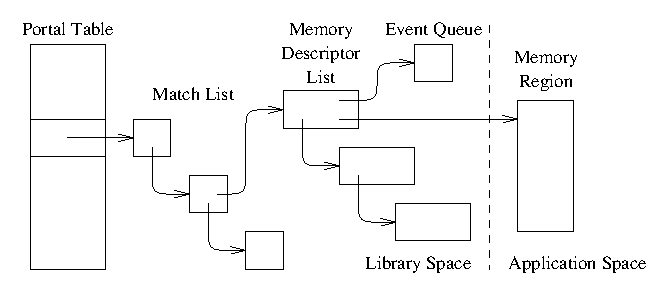
\includegraphics{portals.eps}}
\caption{Portal Addressing Structures}
\label{fig:portals}
\end{figure}

Figure~\ref{fig:flow} illustrates the steps involved in translating a
portal address, starting from the first element in a match list.  If
the match criteria specified in the match list entry are met and the
first entry in the memory descriptor list accepts the
operation\footnote{Memory descriptors can reject operations because
the threshold has been exceeded or due to insufficient space in the
memory region, see Section~\ref{sec:md}}, the operation (put or get)
is performed using the memory region specified in the memory
descriptor.  (Note, while the match list is searched for a matching
entry, only the first element in the memory descriptor list is
considered for the operation.)  If the memory descriptor specifies
that it is to be unlinked after a successful operation, it is unlinked
from the list of memory descriptors.  Next, if the memory descriptor
is unlinked and this empties the memory descriptor list, the match
entry will also be unlinked if its unlink flag has been set.  Finally,
if there is an event queue specified in the memory descriptor, the
operation is logged in the event queue.

\begin{figure}[htbp]
\centerline{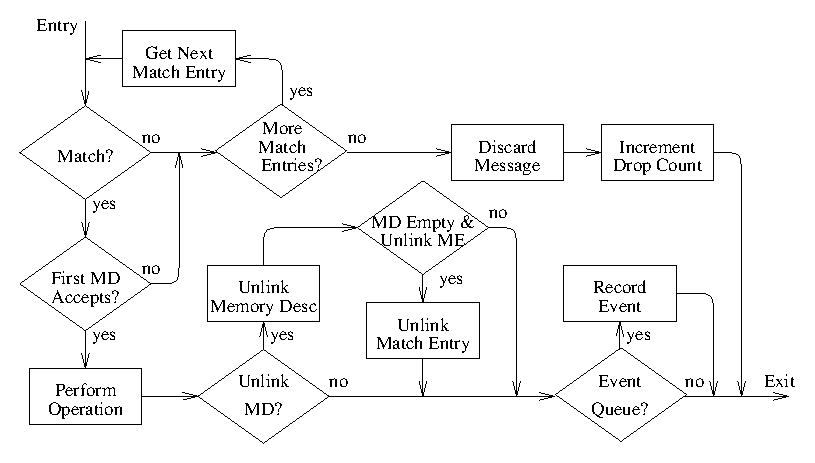
\includegraphics{flow.eps}}
\caption{Portals Address Translation}
\label{fig:flow}
\end{figure}

If the match criteria specified in the match list entry are not met or
the memory descriptor associated with the match list entry rejects the
operation, the address translation continues with the next match list
entry.  If the end of the match list has been reached, the address
translation is aborted and the incoming requested is discarded.

\subsection{Access Control}

A process can control access to its portals using an access control
list.  Each entry in the access control list specifies a process id
and a portal table index.  The access control list is actually an
array of entries.  Each incoming request includes an index into the
access control list (i.e., a ``cookie'' or hint).  If the id of the
process issuing the request doesn't match the id specified in the
access control list entry or the portal table index specified in the
request doesn't match the portal table index specified in the access
control list entry, the request is rejected.

Process identifiers and portal table indexes may include wildcard values to
increase the flexibility of this mechanism.  When the access control
list is initialized, the entry with index zero enables access to all
portals for all processes in the same application and the entry with
index one enables access to all portals for all system processes.  The
remaining entries are set to disable all other access.

Two aspects of this design merit further discussion.  First, the model
assumes that the information in a message header, the sender's id in
particular, is trustworthy.  In most contexts, we assume that the
entity that constructs the header is trustworthy; however, using
cryptographic techniques, we could easily devise a protocol that would
ensure the authenticity of the sender.

Second, because the access check is performed by the receiver, it is
possible that a malicious process will generate thousands of messages
that will be denied by the receiver.  This could saturate the network
and/or the receiver, resulting in a \emph{denial of service} attack.
Moving the check to the sender using capabilities, would remove the
potential for this form of attack.  However, the solution introduces
the complexities of capability management (exchange of capabilities,
revocation, protections, etc).

\section{The Portals API}\label{sec:api}

\subsection{Naming Conventions}\label{sec:conv}
The Portals API defines two types of entities: functions and types.
Function always start with \emph{Ptl} and use mixed upper and lower
case.  When used in the body of this report, function names appear in
italic face, e.g., \emph{PtlInit}.  The functions associated with an
object type will have names that start with \emph{Ptl}, followed by
the two letter object type code shown in Table~\ref{tab:objcodes}.  As
an example, the function \emph{PtlEQAlloc} allocates resources for an
event queue.

\begin{table}[htbp]
  \caption{Object Type Codes}\label{tab:objcodes}
  \medskip
  \begin{center}\small
    \begin{tabular}{lll}
      \emph{xx} & Name & Section \\ \hline
      EQ & Event Queue       & \ref{sec:eq} \\
      MD & Memory Descriptor & \ref{sec:md} \\
      ME & Match Entry       & \ref{sec:me} \\
      NI & Network Interface & \ref{sec:ni} \\
    \end{tabular}
  \end{center}
\end{table}

Type names use lower case with underscores to separate words.  Each
type name starts with \texttt{ptl_} and ends with \texttt{_t}.  When
used in the body of this report, type names appear in a fixed font,
e.g., \texttt{ptl_match_bits_t}.

Names for constants use upper case with underscores to separate words.
Each constant name starts with \texttt{PTL_}.  When used in the body
of this report, type names appear in a fixed font, e.g.,
\texttt{PTL_OK}.

\subsection{Base Types}

The Portals API defines a variety of base types.  These types
represent a simple renaming of the base types provided by the C
programming language.  In most cases these new type names have been
introduced to improve type safety and to avoid issues arising from
differences in representation sizes (e.g., 16-bit or 32-bit integers).

\subsubsection{Sizes}\label{sec:size-t}
The type \texttt{ptl_size_t} is an unsigned integral type used for
representing sizes.

\subsubsection{Handles}\label{sec:handle-type}
Objects maintained by the API are accessed through handles.  Handle
types have names of the form \texttt{ptl_handle_\emph{xx}_t}, where
\emph{xx} is one of the two letter object type codes shown in
Table~\ref{tab:objcodes}.  For example, the type
\texttt{ptl_handle_ni_t} is used for network interface handles.

Each type of object is given a unique handle type to enhance type
checking.  The type, \texttt{ptl_handle_any_t}, can be used when a
generic handle is needed.  Every handle value can be converted into a
value of type \texttt{ptl_handle_any_t} without loss of information.

Handles are not simple values.  Every portals object is associated
with a specific network interface and an identifier for this interface
(along with an object identifier) is part of the handle for the
object.

\subsubsection{Indexes}\label{sec:index-type}
The types \texttt{ptl_pt_index_t} and \texttt{ptl_ac_index_t} are
integral types used for representing portal table indexes and access
control tables indexes, respectively.

\subsubsection{Match Bits}\label{sec:mb-type}
The type \texttt{ptl_match_bits_t} is capable of holding unsigned
64-bit integer values.

\subsubsection{Network Interfaces}\label{sec:ni-type}
The type \texttt{ptl_interface_t} is an integral type used for
identifying different network interfaces.  Users will need to consult
the local documentation to determine appropriate values for the
interfaces available.  The special value \texttt{PTL_IFACE_DEFAULT}
identifies the default interface.

\subsubsection{Identifiers}\label{sec:id-type}
The type \texttt{ptl_id_t} is an integral type used for representing
group ids, node ids, process ids, and rank ids.

\subsubsection{Status Registers}\label{sec:stat-type}
Each network interface maintains an array of status registers that can
be accessed using the \texttt{PtlNIStatus} function (see
Section~\ref{sec:nistatus}).  The type \texttt{ptl_sr_index_t} defines
the types of indexes that can be used to access the status registers.
The only index defined for all implementations is
\texttt{PTL_SR_DROP_COUNT} which identifies the status register that
counts the dropped requests for the interface.  Other indexes (and
registers) may be defined by the implementation.

The type \texttt{ptl_sr_value_t} defines the types of values held in
status registers.  This is a signed integer type.  The size is
implementation dependent, but must be at least 32 bits.

\subsection{Initialization and Cleanup}\label{sec:init}

The Portals API includes a function, \emph{PtlInit}, to initialize the
library and a function, \emph{PtlFini}, to cleanup after the
application is done using the library.

\subsubsection{PtlInit}
\begin{verbatim}
int PtlInit( void );
\end{verbatim}

\noindent
The \emph{PtlInit} function initializes the Portals library.  This
function should be called by all processes in an application before
calling any of the functions defined by the Portal API.  This function
should be called once and only once during initialization by each
process in a parallel job.

\subsubsection*{Return Codes}
\begin{returns}
\item[PTL_OK] Indicates success.
\item[PTL_FAIL] Indicates an error during initialization.
\end{returns}

\subsubsection*{Implementation Notes}
This operation may be implemented as a collective operation involving
all of the processes in a group.

\subsubsection{PtlFini}
\begin{verbatim}
void PtlFini( void );
\end{verbatim}

\noindent
The \emph{PtlFini} function cleans up after the Portals library is no
longer needed by a process.  After this function is called, calls to
any of the functions defined by the Portal API or use of the
structures set up by the Portals API will result in undefined
behavior.  This function should be called once and only once during
termination by each process in a parallel job.  Typically, this
function will be called in the exit sequence of each process.

\subsection{Process Identification}\label{sec:pid}

Processes that use the Portals API, can be identified using a node id
and process id.  Every node in the computing system has a unique node
identifier and every process running on a node has a unique process
identifier.  As such, any process in the computing system can be
identified by its node id and process id.  Processes can also be
identified using a group id and rank id.  When a portals job is
loaded, it is given a unique group identifier. In addition, each
process in the job is assigned a unique rank id starting at zero.

The Portals API defines a type, \texttt{ptl_process_id_t} for
representing process ids using either or both of the schemes, a
function, \emph{PtlGetId}, which can be used to obtain the id of the
current process, and a function, \emph{PtlTransId}, to translate
addresses between the two schemes.

\subsubsection{The Process Id Type}\label{sec:pid-type}
\begin{verbatim}
typedef enum { PTL_ADDR_NID, PTL_ADDR_GID, PTL_ADDR_BOTH } ptl_addr_kind_t;

typedef struct {
    ptl_addr_kind_t addr_kind;   /* kind of address pair */
    ptl_id_t        nid, pid;    /* node id, process id  */
    ptl_id_t        gid, rid;    /* group id, rank id    */
} ptl_process_id_t;
\end{verbatim}

\noindent
The \texttt{ptl_process_id_t} type uses a tag and up to four
identifiers to represent a process id.  Whenever a process id is
filled in by the interface (e.g., by \emph{PtlGetId} or when an event
is recorded), the \texttt{addr_kind} member is set to
\texttt{PTL_ADDR_BOTH}, and all four of the four remaining members
will be set to the appropriate values.  When a process id is passed to
an operation in the Portals API (e.g., \emph{PtlGetId} or
\emph{PtlGet}), the \texttt{addr_kind} member must be
\texttt{PTL_ADDR_NID} or \texttt{PTL_ADDR_GID} and the \texttt{nid}
and \texttt{pid} or \texttt{gid} and \texttt{rid} members must be
filled in, respectively.

\subsubsection{PtlGetId}
\begin{verbatim}
int PtlGetId( ptl_handle_ni_t ni_handle,
              ptl_process_id_t* id,
              ptl_id_t* gsize );
\end{verbatim}

\subsubsection*{Return Codes}
\begin{returns}
\item[PTL_OK] Indicates success.
\item[PTL_NOINIT] Indicates that the Portals API has not been
  successfully initialized.
\item[PTL_SEGV] Indicates that \texttt{id} or \texttt{gsize} is not a
  legal address.
\end{returns}

\subsubsection*{Arguments}
\begin{args}
  handle & input & A network interface handle.\\
  id & output & On successful return, this location will hold the id
  for the calling process.\\
  gsize & output & On successful return, this location will hold the
  number of processes in the process group for this process.
\end{args}

\subsubsection*{Implementation Notes}
Notice that process identifiers are independent of the network
interface(s) used by the process.

\subsubsection{PtlTransId}
\begin{verbatim}
int PtlTransId( ptl_handle_ni_t ni_handle,
                ptl_process_id_t old_id,
                ptl_process_id *new_id );
\end{verbatim}

\subsubsection*{Return Codes}
\begin{returns}
\item[PTL_OK] Indicates success.
\item[PTL_NOINIT] Indicates that the Portals API has not been
  successfully initialized.
\item[PTL_SEGV] Indicates that \texttt{id} is not a legal address.
\item[PTL_ADDR_UNKNOWN] Indicates that the address could not be
  translated.
\end{returns}

\subsubsection*{Arguments}
\begin{args}
  ni_handle & input & A network interface handle.\\
  id & input & The process address to be translated.
  This address should be expressed using nid, pid or gid, rid
  addressing, i.e., \texttt{addr_kind} should be \texttt{PTL_ADDR_NID} 
  or \texttt{PTL_ADDR_GID}.\\
  new_id & output & On successful return, this location will hold a
  process address with all four address members filled in, i.e.,
  \texttt{addr_kind} will be \texttt{PTL_ADDR_BOTH}.
\end{args}

\subsubsection*{Implementation Notes}
This operation should be implemented as a local operation.  That is,
the API should not query other nodes to determine the translation for
a process address.  As a minimum, the API should be able to translate
any addresses for processes in the same group as the calling process.
Other translations can be provided at the discretion of the
implementor.  For example, an implementation may maintain a cache of
recent addresses that it has seen.  (Every incoming message includes
all four addresses for the sending process.)

\subsection{Network Interfaces}\label{sec:ni}
The Portals API supports the use of multiple network interfaces.
However, each interface is treated as an independent entity.
Combining interfaces (e.g., ``bonding'' to create a higher bandwidth
connection) must be implemented by the application or embedded in the
underlying network.  Interfaces are treated as independent entities to
make it easier to cache information on individual network interface
cards.

Once initialized, each interface provides a portal table, an access
control table, and a collection of status registers.  See
Section~\ref{sec:me} for a discussion of updating portal table entries
using the \emph{PtlMEAttach} function.  See Section~\ref{sec:ac} for a
discussion of the initialization and updating of entries in the access
control table.  See Section~\ref{sec:nistatus} for a discussion of the 
\emph{PtlNIStatus} function which can be used to determine the value
of a status register.

Every other type of Portal object (e.g., memory descriptor, event
queue, or match entry) is associated with a specific network
interface.  The association to a network interface is established when
the object is created and is encoded in the handle for the object.

Each network interface is initialized and shutdown independently.  The
initialization routine, \emph{PtlNIInit}, returns a handle for an
interface object which is used in all subsequent portal operations.
The \emph{PtlNIFini} function is used to shutdown an interface and
release any resources that are associated with the interface.

The Portals API also defines the \emph{PtlNIStatus} function to query
the status registers for a network interface, the \emph{PtlNIDist}
function to determine the ``distance'' to another process, and the
\emph{PtlNIHandle} function to determine the network interface that an
object is associated with.

\subsubsection{PtlNIInit}\label{sec:niinit}
\begin{verbatim}
int PtlNIInit( ptl_interface_t  interface,
               ptl_pt_index_t   ptl_size,
               ptl_ac_index_t   acl_size,
               ptl_handle_ni_t* handle );
\end{verbatim}

\noindent 
The \emph{PtlNIInit} function is used to initialized the Portals API
for a network interface.  This function must be called before any
other operations that apply to the interface.  It is an error to
initialize a network interface more than once in the same process.

\subsubsection*{Return Codes}
\begin{returns}
\item[PTL_OK] Indicates success.
\item[PTL_NOINIT] Indicates that the Portals API has not been
  successfully initialized.
\item[PTL_INIT_DUP] Indicates a duplicate initialization of
  \texttt{interface}.
\item[PTL_INIT_INV] Indicates that \texttt{interface} is not a valid
  network interface.
\item[PTL_NOSPACE] Indicates that there is insufficient memory to
  initialize the interface.
\item[PTL_INV_PSIZE] Indicates that \texttt{ptl_size} is invalid.
\item[PTL_INV_ASIZE] Indicates that \texttt{acl_size} is invalid.
\item[PTL_SEGV] Indicates that \texttt{handle} is not a legal address.
\end{returns}

\subsubsection*{Arguments}
\begin{args}
  interface & input & Identifies the network interface to be
  initialized.  (See section~\ref{sec:ni-type} for a discussion of
  values used to identify network interfaces.) \\
  ptl_size & input & Specifies the number of entries in the portal
  table for this interface. \\
  acl_size & input & Specifies the size of the access control list for
  this interface.  (See section~\ref{sec:ac} for more information
  about access control lists.) \\
  handle & output & On successful return, this location will hold a
  handle for the interface.
\end{args}

\subsubsection*{Implementation Notes}
The maximum number of portal table entries allowed by a specific
interface is implementation dependent.  Some portal table indexes may
be reserved by the implementation.  The initialization routine is a
local operation and should not involve communication with any other
nodes.

\subsubsection{PtlNIFini}\label{sec:nifini}
\begin{verbatim}
int PtlNIFini( ptl_handle_ni_t interface );
\end{verbatim}

\noindent
The \emph{PtlNIFini} function is used to release the resources
allocated for a network interface.  Once the \emph{PtlNIFini}
operation has been started, the results of pending API operations
(e.g., operations initiated by another thread) for this interface are
undefined.  Similarly, the effects of incoming operations (puts and
gets) or return values (acknowledgements and replies) for this
interface are undefined.

\subsubsection*{Return Codes}
\begin{returns}
\item[PTL_OK] Indicates success.
\item[PTL_NOINIT] Indicates that the Portals API has not been
  successfully initialized.
\item[PTL_INV_NI] Indicates that \texttt{interface} is not a valid
  network interface handle.
\end{returns}

\subsubsection*{Arguments}
\begin{args}
interface & input & A handle for the interface to shutdown.
\end{args}

\subsubsection{PtlNIBarrier}\label{sec:nibarrier}
\begin{verbatim}
int PtlNIBarrier( ptl_handle_ni_t interface );
\end{verbatim}

\noindent
The \emph{PtlNIBarrier} function blocks the calling process until all
processes in the process group have invoked the \emph{PtlNIBarrier}
function for the specified interface.

\subsubsection*{Return Codes}
\begin{returns}
\item[PTL_OK] Indicates success.
\item[PTL_NOINIT] Indicates that the Portals API has not been
  successfully initialized.
\item[PTL_INV_NI] Indicates that \texttt{interface} is not a valid
  network interface handle.
\end{returns}

\subsubsection*{Arguments}
\begin{args}
interface & input  & A handle for the interface to use. \\
\end{args}

\subsubsection{PtlNIStatus}\label{sec:nistatus}
\begin{verbatim}
int PtlNIStatus( ptl_handle_ni_t interface,
                 ptl_sr_index_t  register,
                 ptl_sr_value_t* status );
\end{verbatim}

\noindent
The \emph{PtlNIStatus} function returns the value of a status register
for the specified interface.  (See section~\ref{sec:stat-type} for
more information on status register indexes and status register
values.)

\subsubsection*{Return Codes}
\begin{returns}
\item[PTL_OK] Indicates success.
\item[PTL_NOINIT] Indicates that the Portals API has not been
  successfully initialized.
\item[PTL_INV_NI] Indicates that \texttt{interface} is not a valid
  network interface handle.
\item[PTL_INV_SR_INDX] Indicates that \texttt{register} is not a valid
  status register.
\item[PTL_SEGV] Indicates that \texttt{status} is not a legal address.
\end{returns}

\subsubsection*{Arguments}
\begin{args}
interface & input  & A handle for the interface to use. \\
register  & input  & An index for the status register to read. \\
status    & output & On successful return, this location will hold the
  current value of the status register. \\
\end{args}

\subsubsection*{Implementation Notes}
The only status register that must be defined is a drop count register
(\texttt{PTL_SR_DROP_COUNT}).  Implementations may define additional
status registers.  Identifiers for the indexes associated with these
registers should start with the prefix \texttt{PTL_SR_}.

\subsubsection{PtlNIDist}
\begin{verbatim}
int PtlNIDist( ptl_handle_ni_t  interface,
               ptl_process_id_t process,
               double*          distance );
\end{verbatim}

\noindent
The \emph{PtlNIDist} function returns the distance to another process
using the specified interface.  Distances are only defined relative to
an interface.  Distance comparisons between different interfaces on
the same node may be meaningless.

\subsubsection*{Return Codes}
\begin{returns}
\item[PTL_OK] Indicates success.
\item[PTL_NOINIT] Indicates that the Portals API has not been
  successfully initialized.
\item[PTL_INV_NI] Indicates that \texttt{interface} is not a valid
  network interface handle.
\item[PTL_INV_PROC] Indicates that \texttt{process} is not a valid
  process identifier.
\item[PTL_SEGV] Indicates that \texttt{distance} is not a legal
  address.
\end{returns}

\subsubsection*{Arguments}
\begin{args}
interface & input  & A handle for the interface to use. \\
process   & input  & An identifier for the process whose distance is being
  requested. \\
distance  & output & On successful return, this location will hold the
  distance to the remote process.
\end{args}

\subsubsection*{Implementation Notes}
This function should return a static measure of distance.  Examples
include minimum latency, the inverse of available bandwidth, or the
number of switches between the two endpoints.

\subsubsection{PtlNIHandle}
\begin{verbatim}
int PtlNIHandle( ptl_handle_any_t handle,
                 ptl_handle_ni_t* interface );
\end{verbatim}

\noindent
The \emph{PtlNIHandle} function returns a handle for the network
interface that the object identified by \texttt{handle} is associated
with.  If the object identified by \texttt{handle} is a network
interface, this function returns the same value it is passed.

\subsubsection*{Return Codes}
\begin{returns}
\item[PTL_OK] Indicates success.
\item[PTL_NOINIT] Indicates that the Portals API has not been
  successfully initialized.
\item[PTL_INV_HANDLE] Indicates that \texttt{handle} is not a valid
  handle.
\item[PTL_SEGV] Indicates that \texttt{interface} is not a legal
  address.
\end{returns}

\subsubsection*{Arguments}
\begin{args}
handle    & input  & A handle for the object. \\
interface & output & On successful return, this location will hold a
  handle for the network interface associated with \texttt{handle}.
\end{args}

\subsubsection*{Implementation Notes}
Every handle should encode the network interface and the object id
relative to this handle.  Both are presumably encoded using integer
values.

\subsection{Match Entries and Match Lists}\label{sec:me}

A match list is a chain of match entries.  Each match entry includes a
list of memory descriptors and a set of match criteria.  The match
criteria can be used to reject incoming requests based on process id
and/or the match bits provided in the request.  A match list is
created using the \emph{PtlMEAttach} function which creates a match
list consisting of a single match entry, attaches the match list to
the specified portal index, and returns a handle for the match entry.
Match entries can be dynamically inserted and removed from a match
list using the \emph{PtlMEInsert} and \emph{PtlMEUnlink} functions.

\subsubsection{PtlMEAttach}\label{sec:meattach}
\begin{verbatim}
typedef enum { PTL_RETAIN, PTL_UNLINK } ptl_unlink_t;

int PtlMEAttach( ptl_handle_ni_t  interface,
                 ptl_pt_index_t   index,
                 ptl_process_id_t matchid,
                 ptl_match_bits_t match_bits,
                 ptl_match_bits_t ignorebits,
                 ptl_unlink_t     unlink,
                 ptl_handle_me_t* handle );
\end{verbatim}

\noindent
Values of the type \texttt{ptl_unlink_t} are used to control whether
an item is unlinked from a list.  The value \texttt{PTL_UNLINK}
enables unlinking.  The value \texttt{PTL_RETAIN} disables unlinking.

The \emph{PtlMEAttach} function creates a match list consisting of a
single entry and attaches this list to the portal table for
\texttt{interface}.  If the portal table already has a match list
attached to the specified index, the existing list (including any
attached memory descriptor lists) must first be unlinked.

\subsubsection*{Return Codes}
\begin{returns}
\item[PTL_OK] Indicates success.
\item[PTL_NOINIT] Indicates that the Portals API has not been
  successfully initialized.
\item[PTL_INUSE] Indicates that the portal table index already has a
match entry attached.
\item[PTL_INV_PTINDEX] Indicates that \texttt{index} is not a valid
  portal table index.
\item[PTL_INV_PROC] Indicates that \texttt{matchid} is not a valid
  process identifier.
\item[PTL_NOSPACE] Indicates that there is insufficient memory to
  allocate the match entry.
\item[PTL_SEGV] Indicates that \texttt{handle} is not a legal address.
\end{returns}

\subsubsection*{Arguments}
\begin{args}
  interface & input  & A handle for the interface to use. \\
  index & input & The portal table index where the match list
  should be attached. \\
  matchid & input & Specifies the match criteria for the process id of
  the requestor.  The constant \texttt{PTL_ID_ANY} can be used to
  wildcard any of the ids in the \texttt{ptl_process_id_t} structure. \\
  match_bits, ignorebits & input & Specify the match criteria to apply
  to the match bits in the incoming request.  The \texttt{ignorebits}
  are used to mask out insignificant bits in the incoming match bits.
  The resulting bits are then compared to the match entry's match bits
  to determine if the incoming request meets the match criteria. \\
  unlink & input & Indicates the match list entry should be unlinked
  when the last memory descriptor associated with this match entry is
  unlinked.  (Note, the check for unlinking a match entry only occurs
  when a memory descriptor is unlinked and this leaves the memory
  descriptor list empty.) \\
  handle & output & On successful return, this location will hold a
  handle for the newly created match entry.
\end{args}

\subsubsection{PtlMEInsert}\label{sec:meinsert}
\begin{verbatim}
typedef enum { PTL_INS_BEFORE, PTL_INS_AFTER } ptl_ins_pos_t;

int PtlMEInsert( ptl_handle_me_t  current,
                 ptl_process_id_t matchid,
                 ptl_match_bits_t match_bits,
                 ptl_match_bits_t ignorebits,
                 ptl_unlink_t     unlink,
                 ptl_ins_pos_t    position,
                 ptl_handle_me_t* handle );
\end{verbatim}

\noindent
Values of the type \texttt{ptl_ins_pos_t} are used to control where a
new item is inserted in a list.  The value \texttt{PTL_INS_BEFORE} is
used to insert the new item before the current item.  The value
\texttt{PTL_INS_AFTER} is used to insert the new item after the
current item.

The \emph{PtlMEInsert} function creates a new match entry and inserts
this entry into the match list containing \texttt{current}.

\subsubsection*{Return Codes}
\begin{returns}
\item[PTL_OK] Indicates success.
\item[PTL_NOINIT] Indicates that the Portals API has not been
  successfully initialized.
\item[PTL_INV_PROC] Indicates that \texttt{matchid} is not a valid
  process identifier.
\item[PTL_INV_ME] Indicates that \texttt{current} is not a valid match
  entry handle.
\item[PTL_ML_TOOLONG] Indicates that the resulting match list is too
  long.  The maximum length for a match list is defined by the
  interface.
\item[PTL_NOSPACE] Indicates that there is insufficient memory to
  allocate the match entry.
\item[PTL_SEGV] Indicates that \texttt{handle} is not a legal address.
\end{returns}

\subsubsection*{Arguments}
\begin{args}
  current & input & A handle for a match entry.  The new match entry
  will be inserted immediately before or immediately after this match
  entry.\\
  matchid, match_bits, ignorebits, unlink & input & See the discussion
  for \emph{PtlMEAttach}.\\ 
  position & input & Indicates whether the new match entry should be
  inserted before or after the \texttt{current} entry.\\
  handle & input & See the discussion for \emph{PtlMEAttach}.\\
\end{args}

\subsubsection{PtlMEUnlink}\label{sec:meunlink}
\begin{verbatim}
int PtlMEUnlink( ptl_handle_me_t entry );
\end{verbatim}

\noindent
The \emph{PtlMEUnlink} function can be used to unlink a match entry
from a match list.  This operation also releases any resources
associated with the match entry (including the list of associated
memory descriptors).  It is an error to use the match entry handle
after calling \emph{PtlMEUnlink}.

\subsubsection*{Return Codes}
\begin{returns}
\item[PTL_OK] Indicates success.
\item[PTL_NOINIT] Indicates that the Portals API has not been
  successfully initialized.
\item[PTL_INV_ME] Indicates that \texttt{entry} is not a valid match
  entry handle.
\end{returns}

\subsubsection*{Arguments}
\begin{args}
entry & input & A handle for the match entry to be unlinked.
\end{args}

\subsection{Memory Descriptors}\label{sec:md}

A memory descriptor contains information about a region of an
application process' memory and an event queue where information about
the operations performed on the memory descriptor are recorded.  The
Portals API provides three operations to create memory descriptors:
\emph{PtlMDAttach}, \emph{PtlMEInsert}, and \emph{PtlMEBind}; an
operation to update a memory descriptor, \emph{PtlMDUpdate}; and an
operation to unlink and release the resources associated with a memory
descriptor, \emph{PtlMDUnlink}.

\subsubsection{The Memory Descriptor Type}\label{sec:md-type}
\begin{verbatim}
typedef struct {
    void*           start;
    ptl_size_t      length;
    int             threshold;
    unsigned int    options;
    void*           user_ptr;
    ptl_handle_eq_t eventq;
} ptl_md_t;
\end{verbatim}

\noindent
The \texttt{ptl_md_t} type defines the application view of a memory
descriptor.  Values of this type are used to initialize and update the
memory descriptors.

\subsubsection*{Members}
\begin{returns}
\item[start, length] Specify the memory region associated with the
  memory descriptor.  The \texttt{start} member specifies the starting
  address for the memory region and the \texttt{length} member
  specifies the length of the region.  The \texttt{start}member can be
  NULL provided that the \texttt{length} member is zero.  (Zero length
  buffers are useful to record events.)  There are no alignment
  restrictions on the starting address or the length of the region;
  although, unaligned messages may be slower (i.e., lower bandwidth
  and/or longer latency) on some implementations.
\item[threshold] Specifies the maximum number of operations that can
  be performed on the memory descriptor.  An operation is any action
  that could possibly generate an event (see Section {sec:ek-type} for
  the different types of events).  In the usual case, the threshold
  value is decremented for each operation on the memory descriptor.
  When the threshold value is zero, the memory descriptor is
  \emph{inactive}, and does not respond to operations.  A memory
  descriptor can have an initial threshold value of zero to allow for
  manipulation of an inactive memory descriptor by the local process.
  A threshold value of \texttt{PTL_MD_THRESH_INF} indicates that there
  is no bound on the number of operations that may be applied to a
  memory descriptor.  Note that local operations (e.g.,
  \emph{PtlMDUpdate}) are not applied to the threshold count. 
\item[options] Specifies the behavior of the memory descriptor.  There
  are five options that can be selected: enable put operations (yes or
  no), enable get operations (yes or no), offset management (local or
  remote), message truncation (yes or no), and acknowledgement (yes or
  no).  Values for this argument can be constructed using a bitwise or
  of the following values:
  \begin{quote}
    \begin{returns}
    \item[PTL_MD_OP_PUT] Specifies that the memory descriptor will
      respond to \emph{put} operations.  By default, memory
      descriptors reject \emph{put} operations.
    \item[PTL_MD_OP_GET] Specifies that the memory descriptor will
      respond to \emph{get} operations.  By default, memory
      descriptors reject \emph{get} operations.
    \item[PTL_MD_MANAGE_REMOTE] Specifies that the offset used in
      accessing the memory region is provided by the incoming request.
      By default, the offset is maintained locally.  When the offset
      is maintained locally, the offset is incremented by the length
      of the request so that the next operation will access the next
      part of the memory region.
    \item[PTL_MD_TRUNCATE] Specifies that the length provided in the
      incoming request can be reduced to match the memory available in
      the region.  (The memory available in a memory region is
      determined by subtracting the offset from the length of the
      memory region.)  By default, if the length in the incoming
      operation is greater than the amount of memory available, the
      operation is rejected.
    \item[PTL_MD_ACK_DISABLE] Specifies that an acknowledgement should
      \emph{not} be sent for incoming \emph{put} operations, even if
      requested.  By default, acknowledgements are sent for \emph{put}
      operations that request an acknowledgement.  Acknowledgements
      are never sent for \emph{get} operations.  The value sent in the
      reply serves as an implicit acknowledgement.
    \end{returns}
  \end{quote}
  
  \textbf{Note}: It is not considered an error to have a memory
  descriptor that does not respond to either \emph{put} or \emph{get}
  operations: Every memory descriptor responds to \emph{reply}
  operations.  Nor is it considered an error to have a memory
  descriptor that responds to both \emph{put} and \emph{get}
  operations.
\item[user_ptr] A user-specified value that is associated with the
  memory descriptor.  The value does not need to be a pointer, but
  must fit in the space used by a pointer.  This value (along with
  other values) is recorded in events associated with operations on
  this memory descriptor.\footnote{Tying the memory descriptor to a
  user-defined value can be useful when multiple memory descriptor
  share the same event queue or when the memory descriptor needs to be
  associated with a data structure maintained by the application.  For
  example, an MPI implementation can set the \texttt{user_ptr}
  argument to the value of an MPI Request.  This direct association
  allows for processing of memory descriptor's by the MPI
  implementation without a table lookup or a search for the
  appropriate MPI Request.}
\item[eventq] A handle for the event queue used to log the operations
  performed on the memory region.  If this argument is
  \texttt{PTl_EQ_NONE}, operations performed on this memory descriptor
  are not logged.
\end{returns}

\subsubsection{PtlMDAttach}\label{sec:mdattach}
\begin{verbatim}
int PtlMDAttach( ptl_handle_me_t  match,
                 ptl_md_t         mem_desc,
                 ptl_unlink_t     unlink,
                 ptl_handle_md_t* handle );
\end{verbatim}

\noindent
The \emph{PtlMDAttach} operation is used to create a memory descriptor
list consisting of a single memory descriptor and attach this list to
a match entry.  If this match entry already has a list of memory
descriptors, the existing memory descriptors must first be unlinked.

\subsubsection*{Return Codes}
\begin{returns}
\item[PTL_OK] Indicates success.
\item[PTL_NOINIT] Indicates that the Portals API has not been
  successfully initialized.
\item[PTL_INUSE] Indicates that \texttt{match} already has a memory
descriptor attached.
\item[PTL_INV_ME] Indicates that \texttt{match} is not a valid
  match entry handle.
\item[PTL_ILL_MD] Indicates that \texttt{mem_desc} is not a legal
  memory descriptor.  This may happen because the memory region
  defined in \texttt{mem_desc} is invalid or because the network
  interface associated with the \texttt{eventq} in \texttt{mem_desc}
  is not the same as the network interface associated with
  \texttt{match}.
\item[PTL_NOSPACE] Indicates that there is insufficient memory to
  allocate the memory descriptor.
\item[PTL_SEGV] Indicates that \texttt{handle} is not a legal address.
\end{returns}

\subsubsection*{Arguments}
\begin{args}
  match & input & A handle for the match entry that the memory
  descriptor will be associated with.\\
  mem_desc & input & Provides initial values for the application
  visible parts of a memory descriptor.  Other than its use for
  initialization, there is no linkage between this structure and the
  memory descriptor maintained by the API. \\
  unlink & input & A flag to indicate whether the memory descriptor is
  unlinked when its threshold drops to zero.  (Note, the check for
  unlinking a memory descriptor only occurs when the threshold
  transitions from one to zero when responding to an operation.  If
  the threshold is set to zero during initialization or using
  \emph{PtlMDUpdate}, the memory descriptor is \textbf{not} unlinked.)
  \\
  handle & output & On successful return, this location will hold a
  handle for the newly created memory descriptor.  The \texttt{handle}
  argument can be NULL, in which case the handle will not be
  returned\footnote{In many cases, the handle will be obtained when an
    event is processed}.
\end{args}

\subsubsection{PtlMDInsert}\label{sec:mdinsert}
\begin{verbatim}
int PtlMDInsert( ptl_handle_md_t  current,
                 ptl_md_t         mem_desc,
                 ptl_unlink_t     unlink,
                 ptl_ins_pos_t    position,
                 ptl_handle_md_t* handle );
\end{verbatim}

\noindent
The \emph{PtlMDInsert} creates a new memory descriptor and links it
into the list containing \texttt{current}.

\subsubsection*{Return Codes}
\begin{returns}
\item[PTL_OK] Indicates success.
\item[PTL_NOINIT] Indicates that the Portals API has not been
  successfully initialized.
\item[PTL_ILL_MD] Indicates that \texttt{mem_desc} is not a legal
  memory descriptor (e.g., the memory region specified by the memory
  descriptor may be invalid).
\item[PTL_INV_MD] Indicates that \texttt{current} is not a valid
  memory descriptor handle.
\item[PTL_NOSPACE] Indicates that there is insufficient memory to
  allocate the memory descriptor.
\item[PTL_SEGV] Indicates that \texttt{handle} is not a legal address.
\end{returns}

\subsubsection*{Arguments}
\begin{args}
  current & input & A handle for a memory descriptor.  The new memory
  descriptor will be inserted immediately before or immediately after
  this memory descriptor.\\
  mem_desc, unlink & input & See the discussion for \emph{PtlMDAttach}. \\
  position & input & Indicates whether the new memory descriptor
  should be inserted before or after the \texttt{current} entry. \\
  handle & output & See the discussion for \emph{PtlMDAttach}.
\end{args}

\subsubsection{PtlMDBind}\label{sec:mdbind}
\begin{verbatim}
int PtlMDBind( ptl_handle_ni_t  interface,
               ptl_md_t         mem_desc,
               ptl_handle_md_t* handle );
\end{verbatim}

\noindent
The \emph{PtlMDBind} operation is used to create a ``free floating''
memory descriptor, i.e., a memory descriptor that is not part of the
memory descriptor list for a match entry.

\subsubsection*{Return Codes}
\begin{returns}
\item[PTL_OK] Indicates success.
\item[PTL_NOINIT] Indicates that the Portals API has not been
  successfully initialized.
\item[PTL_INV_NI] Indicates that \texttt{interface} is not a valid
  match entry handle.
\item[PTL_ILL_MD] Indicates that \texttt{mem_desc} is not a legal
  memory descriptor.  This may happen because the memory region
  defined in \texttt{mem_desc} is invalid or because the network
  interface associated with the \texttt{eventq} in \texttt{mem_desc}
  is not the same as the network interface, \texttt{interface}.
\item[PTL_NOSPACE] Indicates that there is insufficient memory to
  allocate the memory descriptor.
\item[PTL_SEGV] Indicates that \texttt{handle} is not a legal address.
\end{returns}

\subsubsection*{Arguments}
\begin{args}
  interface & input & A handle for the network interface that the
  memory descriptor will be associated with.\\
  mem_desc & input & Provides initial values for the application
  visible parts of a memory descriptor.  Other than its use for
  initialization, there is no linkage between this structure and the
  memory descriptor maintained by the API. \\
  handle & output & On successful return, this location will hold a
  handle for the newly created memory descriptor.  The \texttt{handle}
  argument must be a valid address and cannot be NULL.
\end{args}

\subsubsection{PtlMDUnlink}\label{sec:mdfree}
\begin{verbatim}
int PtlMDUnlink( ptl_handle_md_t mem_desc );
\end{verbatim}

\noindent
The \emph{PtlMDUnlink} function unlinks the memory descriptor from any
memory descriptor list it may be linked to and releases the resources
associated with a memory descriptor.  (This function does not free the
memory region associated with the memory descriptor.)

\subsubsection*{Return Codes}
\begin{returns}
\item[PTL_OK] Indicates success.
\item[PTL_NOINIT] Indicates that the Portals API has not been
  successfully initialized.
\item[PTL_INV_MD] Indicates that \texttt{mem_desc} is not a valid
  memory descriptor handle.
\end{returns}

\subsubsection*{Arguments}
\begin{args}
  mem_desc & input & A handle for the memory descriptor to be
  released.
\end{args}


\subsubsection{PtlMDUpdate}\label{sec:mdupdate}
\begin{verbatim}
int PtlMDUpdate( ptl_handle_md_t mem_desc,
                 ptl_md_t*       old,
                 ptl_md_t*       new,
                 ptl_handle_eq_t testq );
\end{verbatim}

\noindent
The \emph{PtlMDUpdate} function provides a conditional, atomic update
operation for memory descriptors.  If \texttt{old} is not NULL, the
current value of the memory descriptor identified by \texttt{mem_desc}
is recorded in the location identified by \texttt{old}.  If
\texttt{new} is not NULL the memory descriptor identified by handle
will be updated to reflect the values in the structure pointed to by
\texttt{new} if \texttt{testq} has the value \texttt{PTL_EQ_NONE} or
if the event queue identified by \texttt{testq} is empty.

\subsubsection*{Return Codes}
\begin{returns}
\item[PTL_OK] Indicates success.
\item[PTL_NOINIT] Indicates that the Portals API has not been
  successfully initialized.
\item[PTL_NOUPDATE] Indicates that the update was not performed
  because \texttt{testq} was not empty.
\item[PTL_INV_MD] Indicates that \texttt{mem_desc} is not a valid
  memory descriptor handle.
\item[PTL_ILL_MD] Indicates that the value pointed to by \texttt{new}
  is not a legal memory descriptor (e.g., the memory region specified
  by the memory descriptor may be invalid).
\item[PTL_INV_EQ] Indicates that \texttt{testq} is not a valid event
  queue handle.
\item[PTL_SEGV] Indicates that \texttt{new} or \texttt{old} is not a
  legal address.
\end{returns}

\subsubsection*{Arguments}
\begin{args}
  mem_desc & input & A handle for the memory descriptor to update. \\
  old & output & If \texttt{old} is not the value \texttt{NULL}, the
  current value of the memory descriptor will be stored in the
  location identified by \texttt{old}.\\
  new & input & If \texttt{new} is not the value \texttt{NULL}, this
  argument provides the new values for the memory descriptor, if the
  update is performed. \\
  testq & input & A handle for an event queue used to predicate the
  update.  If \texttt{testq} is equal to \texttt{PTL_EQ_NONE}, the
  update is performed unconditionally.  Otherwise, the update is
  performed if and only if \texttt{testq} is empty.  If the update is
  not performed, the function returns the value \texttt{PTL_NOUPDATE}.
  (Note, the \texttt{testq} argument does not need to be the same as
  the event queue associated with the memory descriptor.)
\end{args}

The conditional update can be used to ensure that the memory
descriptor has not changed between the time it was examined and the
time it is updated.  In particular, it is needed to support an MPI
implementation where the activity of searching an unexpected message
queue and posting a receive must be atomic.

\subsection{Events and Event Queues}\label{sec:eq}

Event queues are used to log operations performed on memory
descriptors.  They can also be used to hold acknowledgements for
completed \emph{put} operations and to note when the data specified in
a \emph{put} operation has been sent (i.e., when it is safe to reuse
the buffer that holds this data).  Multiple memory descriptors can
share a single event queue.

In addition to the \texttt{ptl_handle_eq_t} type, the Portals API
defines two types associated with events: The
\texttt{ptl_event_kind_t} type defines the kinds of events that can be
stored in an event queue.  The \texttt{ptl_event_t} type defines a
structure that holds the information associated with an event.

The Portals API also provides five functions for dealing with event
queues: The \emph{PtlEQAlloc} function is used to allocate the API
resources needed for an event queue, the \emph{PtlEQFree} function is
used to release these resources, the \emph{PtlEQCount} function can be
used to obtain the number of events in an event queue, the
\emph{PtlEQGet} function can be used to get the next event from an
event queue, and the \emph{PtlEQWait} function can be used to block a
process (or thread) until an event queue has at least one event.

\subsubsection{Kinds of Events}\label{sec:ek-type}
\begin{verbatim}
typedef enum { 
    PTL_EVENT_GET,
    PTL_EVENT_PUT,
    PTL_EVENT_REPLY,
    PTL_EVENT_ACK,
    PTL_EVENT_SENT
} ptl_event_kind_t;
\end{verbatim}

\noindent
The Portals API defines five types of events that can be logged in an
event queue:
\begin{returns}
\item[PTL_EVENT_GET] A remote \emph{get} operation was performed on
  the memory descriptor.  This event is logged after the reply has
  been sent by the local node.  As such, the process could free the
  memory descriptor once it sees this event.
\item[PTL_EVENT_PUT] A remote \emph{put} operation was performed on
  the memory descriptor.  This event is logged after the data (if any)
  is written into the memory descriptor and after the acknowledgement
  (if any) has been sent.
\item[PTL_EVENT_REPLY] A \emph{reply} has been received for the memory
  descriptor.  This event is logged after the data (if any) from the
  reply has been written into the memory descriptor.
\item[PTL_EVENT_ACK] An \emph{acknowledgement} was received.  This
  event is logged when the acknowledgement is received
\item[PTL_EVENT_SENT] An outgoing buffer was sent (see
  Section~\ref{sec:put}).  This event is logged after the entire
  buffer has been sent and it is safe for the application to reuse the
  buffer.
\end{returns}

\subsubsection{The Event Type}\label{sec:event-type}
\begin{verbatim}
typedef struct {
    ptl_event_kind_t      type;
    unsigned int          sequence;
    ptl_process_id_t      initiator;
    ptl_pt_index_t        portal;
    ptl_match_bits_t      match_bits;
    ptl_size_t            rlength;
    ptl_size_t            mlength;
    ptl_size_t            offset;
    ptl_md_t              mem_desc;
    ptl_hdr_data_t        hdr_data;
} ptl_event_t;
\end{verbatim}

\noindent
An event structure includes the following members:
\begin{returns}
\item[type] Indicates the type of operation that generated the event.
\item[sequence] The sequence number of the event.
\item[initiator] The id of the initiator (group id, rank id).
\item[portal] The portal table index specified in the request.
\item[match_bits] A copy of the match bits specified in the request.
  See section~\ref{sec:me} for more information on match bits.
\item[rlength] The length (in bytes) specified in the request.
\item[mlength] The length (in bytes) of the data that was manipulated
  by the operation.  For truncated operations, the manipulated length
  will be the number of bytes specified by the memory descriptor
  (possibly with an offset) operation.  For all other operations, the
  manipulated length will be the length of the requested operation.
\item[offset] Is the displacement (in bytes) into the memory region
  that the operation used.  The offset can be determined by the
  operation (see Section~\ref{sec:datamovement}) for a remote managed
  memory descriptor, or by the local memory descriptor (see
  Section~\ref{sec:md}).
\item[mem_desc] Is a copy of the memory descriptor immediately after
  the event has been processed.
\item[hdr_data] 64 bits of out-of-band user data (see
  Section~\ref{sec:put}).
\end{returns}

\subsubsection{PtlEQAlloc}\label{sec:eqalloc}
\begin{verbatim}
int PtlEQAlloc( ptl_handle_ni_t  interface,
                ptl_size_t       count,
                ptl_handle_eq_t* handle );
\end{verbatim}

\noindent
The \emph{PtlEQAlloc} function is used to build an event queue.
\subsubsection*{Return Codes}
\begin{returns}
\item[PTL_OK] Indicates success.
\item[PTL_NOINIT] Indicates that the Portals API has not been
  successfully initialized.
\item[PTL_INV_NI] Indicates that \texttt{interface} is not a valid
  network interface handle.
\item[PTL_NOSPACE] Indicates that there is insufficient memory to
  allocate the event queue.
\item[PTL_SEGV] Indicates that \texttt{handle} is not a legal address.
\end{returns}

\subsubsection*{Arguments}
\begin{args}
  interface & input & A handle for the interface that the event queue
  will be associated with. \\
  count & input & The number of events that can be stored in the event
  queue.\\
  handle & output & On successful return, this location will hold a
  handle for the newly created event queue.
\end{args}

\subsubsection{PtlEQFree}\label{sec:eqfree}
\begin{verbatim}
int PtlEQFree( ptl_handle_eq_t eventq );
\end{verbatim}

\noindent
The \emph{PtlEQFree} function releases the resources associated with
an event queue.  This function does not free the memory region
associated with the event queue.  It is up to the user to insure that
no memory descriptors are associated with the event queue once it is
freed.
\subsubsection*{Return Codes}
\begin{returns}
\item[PTL_OK] Indicates success.
\item[PTL_NOINIT] Indicates that the Portals API has not been
  successfully initialized.
\item[PTL_INV_EQ] Indicates that \texttt{eventq} is not a valid event
  queue handle.
\end{returns}

\subsubsection*{Arguments}
\begin{args}
eventq & input & A handle for the event queue to be released.
\end{args}

\subsubsection{PtlEQCount}\label{sec:eqlast}
\begin{verbatim}
int PltEQCount( ptl_handle_eq_t eventq,
                ptl_size_t*     count );
\end{verbatim}

\noindent
The \emph{PTLEQCount} function can be used to discover the number
events in an event queue.

\subsubsection*{Return Codes}
\begin{returns}
\item[PTL_OK] Indicates success.
\item[PTL_NOINIT] Indicates that the Portals API has not been
  successfully initialized.
\item[PTL_INV_EQ] Indicates that \texttt{eventq} is not a valid event
  queue handle.
\item[PTL_SEGV] Indicates that \texttt{count} is not a legal address.
\end{returns}

\subsubsection*{Arguments}
\begin{args}
  eventq & input & A handle for the event queue. \\
  count & output & On successful return, this location will hold the
  number of events in the event queue.
\end{args}

\subsubsection{PtlEQGet}\label{sec:eqget}
\begin{verbatim}
int PltEQGet( ptl_handle_eq_t eventq,
              ptl_event_t*    event );
\end{verbatim}

\noindent
The \emph{PTLEQGet} function is a nonblocking function that can be
used to get the next event in an event queue.  The event is removed
from the queue.

\subsubsection*{Return Codes}
\begin{returns}
\item[PTL_OK] Indicates success.
\item[PTL_EQ_DROPPED] Indicates success (i.e., an event is returned)
  and that at least one event between this event and the last event
  obtained (using \emph{PtlEQGet} or \emph{PtlEQWait}) from this event
  queue has been dropped due to limited space in the event queue.
\item[PTL_NOINIT] Indicates that the Portals API has not been
  successfully initialized.
\item[PTL_EQ_EMPTY] Indicates that \texttt{eventq} is empty.
\item[PTL_INV_EQ] Indicates that \texttt{eventq} is not a valid event
  queue handle.
\item[PTL_SEGV] Indicates that \texttt{event} is not a legal address.
\end{returns}

\subsubsection*{Arguments}
\begin{args}
  eventq & input & A handle for the event queue.\\
  event & output& On successful return, this location will hold the
  values associated with the next event in the event queue.
\end{args}

\subsubsection{PtlEQWait}\label{sec:eqwait}
\begin{verbatim}
int PltEQWait( ptl_handle_eq_t eventq,
               ptl_event_t*    event );
\end{verbatim}

\noindent
The \emph{PTLEQWait} function can be used to block the calling process
(thread) until there is an event in an event queue.  This function
also returns the next event in the event queue and removes this event
from the queue.  This is the only blocking operation in the Portals
3.0 API.

\subsubsection*{Return Codes}
\begin{returns}
\item[PTL_OK] Indicates success.
\item[PTL_EQ_DROPPED] Indicates success (i.e., an event is returned)
  and that at least one event between this event and the last event
  obtained (using \emph{PtlEQGet} or \emph{PtlEQWait}) from this event
  queue has been dropped due to limited space in the event queue.
\item[PTL_NOINIT] Indicates that the Portals API has not been
  successfully initialized.
\item[PTL_INV_EQ] Indicates that \texttt{eventq} is not a valid event
  queue handle.
\item[PTL_SEGV] Indicates that \texttt{event} is not a legal address.
  queue handle.
\end{returns}

\subsubsection*{Arguments}
\begin{args}
  eventq & input & A handle for the event queue to wait on.  The
  calling process (thread) will be blocked until \texttt{eventq} is
  not empty.\\
  event & output & On successful return, this location will hold the
  values associated with the next event in the event queue.
\end{args}

\subsection{The Access Control Table}\label{sec:ac}

Processes can use the access control table to control which processes
are allowed to perform operations on portal table entries.  Each
communication interface has a portal table and an access control
table.  The access control table for the default interface contains an
entry at index zero that allows all members of the same group to
communicate.  Entries in the access control table can be manipulated
using the \emph{PtlACEntry} function.

\subsubsection{PtlACEntry}\label{sec:acentry}
\begin{verbatim}
int PtlACEntry( ptl_handle_ni_t interface,
                ptl_ac_index_t  index,
                ptl_processid_t matchid,
                ptl_pt_index_t  portal );
\end{verbatim}

\noindent
The \emph{PtlACEntry} function can be used to update an entry in the
access control table for an interface.

\subsubsection*{Return Codes}
\begin{returns}
\item[PTL_OK] Indicates success.
\item[PTL_NOINIT] Indicates that the Portals API has not been
  successfully initialized.
\item[PTL_INV_NI] Indicates that \texttt{interface} is not a valid
  network interface handle.
\item[PTL_AC_INV_INDEX] Indicates that \texttt{index} is not a valid
  access control table index.
\item[PTL_INV_PROC] Indicates that \texttt{matchid} is not a valid
  process identifier.
\item[PTL_PT_INV_INDEX] Indicates that \texttt{portal} is not a valid
  portal table index.
\end{returns}

\subsubsection*{Arguments}
\begin{args}
  interface & input & Identifies the interface to use. \\
  index & input & The index of the entry in the access control table
  to update. \\
  matchid & input & Identifies the process(es) that are allowed to
  perform operations.  The value \texttt{PTL_ID_ANY} can be used to
  wildcard either or both components of the process identifier. \\
  portal & input & Identifies the portal index(es) that can be used.
  The value \texttt{PTL_PT_INDEX_ANY} can be used to wildcard the
  portal index.
\end{args}

\subsection{Data Movement Operations}\label{sec:datamovement}

The Portals API provides two data movement operations: \emph{PtlPut}
and \emph{PtlGet}.

\subsubsection{PtlPut}\label{sec:put}
\begin{verbatim}
typedef enum { PTL_ACK_REQ, PTL_NOACK_REQ } ptl_ack_req_t;

int PtlPut( ptl_handle_md_t  mem_desc,
            ptl_ack_req_t    ack_req,
            ptl_process_id_t target,
            ptl_pt_index_t   portal,
            ptl_ac_index_t   cookie,
            ptl_match_bits_t match_bits,
            ptl_size_t       offset,
            ptl_hdr_data_t   hdr_data );
\end{verbatim}

\noindent
Values of the type \texttt{ptl_ack_req_t} are used to control whether
an acknowledgement should be sent when the operation completes (i.e.,
when the data has been written to a memory descriptor of the
\texttt{target} process).  The value \texttt{PTL_ACK_REQ} requests an
acknowledgement, the value \texttt{PTL_NOACK_REQ} requests that no
acknowledgement should be generated.

The \emph{PtlPut} function initiates an asynchronous put operation.
There are two significant events associated with a put operation:
completion of the send by the local node (\texttt{PTL_EVENT_SENT}) and
the receipt of an acknowledgement (\texttt{PTL_EVENT_ACK}) indicating
that the operation was accepted by the target.  These events will be
logged in the event queue associated with the memory descriptor
(\texttt{mem_desc}) used in the put operation.  Using a memory
descriptor that does not have an associated event queue results in
these events being discarded.  In this case, the application must have
another mechanism (e.g., a higher level protocol) for determining when
it is safe to modify the memory region associated with the memory
descriptor.

\subsubsection*{Return Codes}
\begin{returns}
\item[PTL_OK] Indicates success.
\item[PTL_NOINIT] Indicates that the Portals API has not been
  successfully initialized.
\item[PTL_INV_MD] Indicates that \texttt{mem_desc} is not a valid
  memory descriptor.
\item[PTL_INV_PROC] Indicates that \texttt{target} is not a valid
  process id.
\end{returns}

\subsubsection*{Arguments}
\begin{args}
  mem_desc & input & A handle for the memory descriptor that describes
  the memory to be sent.  If the memory descriptor has an event queue
  associated with it, it will be used to record an event when the
  message has been sent (\texttt{PTL_EVENT_SENT}). \\
  ack_req & input & Controls whether an acknowledgement event is
  requested.  Acknowledgements are only sent when they are requested
  by the initiating process \textbf{and} the memory descriptor has an
  event queue \textbf{and} the target memory descriptor enables them.\\
  target & input & A process id for the target process.\\
  portal & input & The index in the remote portal table.\\
  cookie & input & The index into the access control table of the
  target process.\\
  match_bits & input & The match bits to use for message selection at
  the target process.\\
  offset & input & The offset into the target memory descriptor (only
  used when the target memory descriptor has the
  \texttt{PTL_MD_MANAGE_REMOTE} option set).\\
  hdr_data & input & 64 bits of user data that can be included in
  message header.  This data is written to an event queue entry at the
  target if an event queue is present on the matching memory
  descriptor.
\end{args}

\subsubsection{PtlGet}\label{sec:get}
\begin{verbatim}
int PtlGet( ptl_handle_md_t  mem_desc,
            ptl_process_id_t target,
            ptl_pt_index_t   portal,
            ptl_ac_index_t   cookie,
            ptl_match_bits_t match_bits,
            ptl_size_t       offset );
\end{verbatim}

\noindent
The \emph{PtlGet} function initiates a remote read operation.

\subsubsection*{Return Codes}
\begin{returns}
\item[PTL_OK] Indicates success.
\item[PTL_NOINIT] Indicates that the Portals API has not been
  successfully initialized.
\item[PTL_INV_MD] Indicates that \texttt{mem_desc} is not a valid
  memory descriptor.
\item[PTL_INV_PROC] Indicates that \texttt{target} is not a valid
  process id.
\end{returns}

\subsubsection*{Arguments}
\begin{args}
  mem_desc & input & A handle for the memory descriptor that describes
  the memory into which the requested data will be received.  The
  memory descriptor can have an event queue associated with it to
  record events, such as when the message has been received
  (\texttt{PTL_EVENT_REPLY}).\\
  target & input & A process id for the target process.\\
  portal & input & The index in the remote portal table.\\
  cookie & input & The index into the access control table of the
  target process.\\
  match_bits & input & The match bits to use for message selection at
  the target process.\\
  offset & input & The offset into the target memory descriptor
  (ignored unless the target memory descriptor has the
  \texttt{PTL_MD_MANAGE_REMOTE} option set).
\end{args}

\subsection{Summary}
We conclude this section by summarizing the names introduced by the
Portals 3.0 API.  We start by summarizing the names of the types
introduced by the API.  This is followed by a summary of the functions
introduced by the API.  Which is followed by a summary of the function
return codes.  Finally, we conclude with a summary of the other
constant values introduced by the API.

Table~\ref{tab:types} presents a summary of the types defined by the
Portals API.  The first column in this table gives the type name, the
second column gives a brief description of the type, the third column
identifies the section where the type is defined, and the fourth
column lists the functions that have arguments of this type.

\begin{table}[htbp]
  \caption{Types Defined by the Portals 3.0 API}\label{tab:types}
  \medskip
  \begin{center}\small
    \begin{tabular}%
      {>{\ttfamily\makeunderletter}l%
        l%
        l%
        >{\PreserveBackslash\raggedright\hspace{0pt}}p{1.95in}}
      \textrm{Name}    & Meaning & Section & Functions \\ \hline
      ptl_ac_index_t   & indexes for an access control table &
         \ref{sec:index-type} & PtlACEntry, PtlPut, PtlGet \\
      ptl_ack_req_t    & acknowledgement request types & \ref{sec:put} 
         & PtlPut \\
      ptl_addr_kind_t  & kinds of process addresses (nid, pid or gid,
         rid) & \ref{sec:pid-type} & \\
      ptl_event_kind_t & kinds of events (get, put, reply, etc.) &
         \ref{sec:ek-type} & PtlGetId \\
      ptl_event_t      & information about events &
         \ref{sec:event-type} & PtlEQGet \\
      ptl_handle_any_t  & handles for any object & 
         \ref{sec:handle-type} & PtlNIHandle \\ 
      ptl_handle_eq_t  & handles for event queues & 
         \ref{sec:handle-type} & PtlEQAlloc, PtlEQFree,
         PtlEQCount, PtlEQGet, PtlEQWait, PtlMDUpdate \\ 
      ptl_handle_md_t  & handles for memory descriptors &
         \ref{sec:handle-type} & PtlMDAlloc, PtlMDUnlink, PtlMDUpdate,
         PtlMEAttach, PtlMEInsert, PtlPut, PtlGet \\
      ptl_handle_me_t  & handles for match entries & 
         \ref{sec:handle-type} & PtlMEAttach, PtlMEInsert, PtlMEUnlink
         \\
      ptl_handle_ni_t  & handles for network interfaces &
         \ref{sec:handle-type} & PtlNIInit, PtlNIFini, PtlNIStatus,
         PtlNIDist, PtlEQAlloc, PtlACEntry, PtlPut, PtlGet 
         \\ 
      ptl_id_t & identifiers (nid, pid, gid, rid) & \ref{sec:id-type} & \\
      ptl_ins_pos_t    & insertion position (before or after) &
         \ref{sec:meinsert} & PtlMeInsert, PtlMDInsert \\
      ptl_interface_t  & identifiers for network interfaces &
         \ref{sec:ni-type} & PtlNIInit \\
      ptl_match_bits_t & match (and ignore) bits & 
         \ref{sec:mb-type} & PtlMEAttach, PtlMEInsert, PtlPut, PtlGet
         \\ 
      ptl_md_t         & memory descriptors & 
         \ref{sec:md-type} & PtlMDAttach, PtlMDInsert, PtlMDUpdate \\
      ptl_process_id_t & process identifiers & 
         \ref{sec:pid-type} & PtlGetId, PtlNIDist, PtlMEAttach,
         PtlACEntry, PtlPut, PtlGet \\
      ptl_pt_index_t   & indexes for portal tables &
         \ref{sec:index-type} & PtlMEAttach, PtlACEntry \\
      ptl_size_t       & sizes & \ref{sec:size-t} & PtlEQAlloc,
         PtlEQCount, PtlPut, PtlGet \\
      ptl_sr_index_t   & indexes for status registers &
         \ref{sec:stat-type} & PtlNIStatus \\
      ptl_sr_value_t   & values in status registers &
         \ref{sec:stat-type} & PtlNIStatus \\
      ptl_unlink_t     & unlink options & \ref{sec:meattach} &
         PtlMEAttach, PtlMEInsert, PtlMDAttach, PtlMDInsert \\
     \end{tabular}
  \end{center}
\end{table}

Table~\ref{tab:func} presents a summary of the functions defined by
the Portals API.  The first column in this table gives the name for
the function, the second column gives a brief description of the
operation implemented by the function, and the third column identifies
the section where the function is defined.

\begin{table}[htbp]
  \caption{Functions Defined by the Portals 3.0 API}\label{tab:func}
  \medskip
  \begin{center}\small
    \begin{tabular}%
      {l%
%        >{\PreserveBackslash\raggedright\hspace{0pt}}p{3.5in}%
        l%
       l}%
      Name & Operation & Section \\ \hline
      PtlACEntry  & update an entry in an access control table &
         \ref{sec:ac} \\
      PtlEQAlloc  & create an event queue & \ref{sec:eq} \\
      PtlEQCount   & get the number events in an event queue &
         \ref{sec:eq} \\
      PtlEQGet   & get the next event from an event queue &
         \ref{sec:eq} \\
      PtlEQFree   & release the resources for an event queue &
         \ref{sec:eq} \\
      PtlEQWait   & wait for a new event in an event queue &
         \ref{sec:eq} \\
      PtlFini     & shutdown the Portals API & \ref{sec:init} \\
      PtlGet      & perform a get operation & \ref{sec:datamovement} \\
      PtlGetId    & get the id for the current process & \ref{sec:pid} \\
      PtlInit     & initialize the Portals API & \ref{sec:init} \\
      PtlMDAttach & create a memory descriptor and attach it to a
         match entry & \ref{sec:md} \\
      PtlMDBind   & create a free-floating memory descriptor &
         \ref{sec:mdbind} \\
      PtlMDInsert & create a memory descriptor and insert it in a
         list & \ref{sec:md} \\
      PtlMDUnlink   & remove a memory descriptor from a list and
         release its resources & \ref{sec:md} \\
      PtlMDUpdate & update a memory descriptor & \ref{sec:md} \\
      PtlMEAttach & create a match entry and attach it to a portal
        table & \ref{sec:me} \\
      PtlMEInsert & create a match entry and insert it in a list &
         \ref{sec:me} \\
      PtlMEUnlink & remove a match entry from a list and release its
         resources & \ref{sec:me} \\
      PtlNIBarrier& barrier synchronization for a process group & \ref{sec:ni} \\
      PtlNIDist   & get the distance to another process & \ref{sec:ni} \\
      PtlNIFini   & shutdown a network interface & \ref{sec:ni} \\
      PtlNIHandle & get the network interface handle for an object 
         & \ref{sec:ni} \\
      PtlNIInit   & initialize a network interface & \ref{sec:ni} \\
      PtlNIStatus & read a network interface status register & \ref{sec:ni} \\
      PtlPut      & perform a put operation & \ref{sec:datamovement} \\
      PtlTransId  & translate id & \ref{sec:pid} \\
    \end{tabular}
  \end{center}
\end{table}

Table~\ref{tab:retcodes} summarizes the return codes used by functions
defined by the Portals API.  All of these constants are integer
values.  The first column of this table gives the symbolic name for
the constant, the second column gives a brief description of the
value, and the third column identifies the functions that can return
this value.

\begin{table}[htbp]
  \caption{Function Return Codes for the Portals 3.0 API}\label{tab:retcodes}
  \medskip
  \begin{center}\small
    \begin{tabular}%
      {>{\ttfamily\makeunderletter}l%
        l%
        >{\PreserveBackslash\raggedright\hspace{0pt}}p{2.5in}}
      \textrm{Name}   & Meaning & Functions \\ \hline
      PTL_AC_INV_INDEX & invalid access control table index &
         PtlACEntry \\
      PTL_ADDR_UNKNOWN & unknown process address & PtlTransId \\
      PTL_EQ_DROPPED  & at least one event has been dropped &
      PtlEQGet, PtlWait \\
      PTL_EQ_EMPTY    & no events available in an event queue &
         PltEQGet \\
      PTL_FAIL        & error during initialization or cleanup &
         PtlInit, PtlFini \\
      PTL_ILL_MD      & illegal memory descriptor values &
         PtlMDAttach, PtlMDInsert, PtlMDBind, PtlMDUpdate \\
      PTL_INIT_DUP    & duplicate initialization of an interface &
         PtlNIInit \\
      PTL_INIT_INV    &  initialization of an invalid interface &
         PtlNIInit \\
      PTL_INV_ASIZE   & invalid access control table size &
         PtlNIInit \\
      PTL_INV_EQ      & invalid event queue handle &
         PtlMDUpdate, PtlEQFree, PtlEQCount, PtlEQGet \\
      PTL_INV_HANDLE  & invalid handle &
         PtlNIHandle \\
      PTL_INV_MD      & invalid memory descriptor handle &
         PtlMDInsert, PtlMDUnlink, PtlMDUpdate \\
      PTL_INV_ME      & invalid match entry handle & PtlMDAttach,
         PtlMDInsert \\
      PTL_INV_NI      & invalid network interface handle &
         PtlNIBarrier, PtlNIDist, PtlNIFini, PtlMDBind, PtlEQAlloc \\
      PTL_INV_PROC    & invalid process identifier &
          PtlNIDist, PtlMEAttach, PtlMEInsert, PtlACEntry, PtlPut,
          PtlGet \\
      PTL_INV_PSIZE   & invalid portal table size &
         PtlNIInit \\
      PTL_INV_PTINDEX & invalid portal table index &
         PtlMEAttach \\
      PTL_INV_REG     & invalid status register &
          PtlNIStatus \\
      PTL_INV_SR_INDX & invalid status register index &
         PtlNIStatus \\
      PTL_ML_TOOLONG  & match list too long &
         PtlMEInsert \\
      PTL_NOINIT     & uninitialized API & \emph{all}, except PtlInit \\
      PTL_NOSPACE     & insufficient memory &
         PtlNIInit, PtlMDAttach, PtlMDInsert, PtlMDBind, PtlEQAlloc,
         PtlMEAttach, PtlMEInsert \\
      PTL_NOUPDATE    & no update was performed & 
         PtlMDUpdate \\
      PTL_OK          & success & \emph{all} \\
      PTL_SEGV        & addressing violation &
         PtlGetId, PtlTransId, PtlNIInit, PtlNIStatus, PtlNIDist,
         PtlNIHandle, PtlMEAttach, PtlMEInsert, PtlMDAttach,
         PtlMDInsert, PtlMDBind, PtlMDUpdate, PtlEQAlloc, PtlEQCount,
         PtlEQGet, PtlEQWait \\
    \end{tabular}
  \end{center}
\end{table}

Table~\ref{tab:oconsts} summarizes the remaining constant values
introduced by the Portals API.  The first column in this table
presents the symbolic name for the constant, the second column gives a 
brief description of the value, the third column identifies the type
for the value, and the fourth column identifies the sections in which
the value is mentioned.

\begin{table}[htbp]
  \caption{Other Constants Defined by the Portals 3.0 API}\label{tab:oconsts}
  \medskip
  \begin{center}\small
    \begin{tabular}%
      {>{\ttfamily\makeunderletter}l%
        l%
        >{\ttfamily\makeunderletter}l%
        l}
      \textrm{Name}   & Meaning & Base type & Section \\ \hline
      PTL_ACK_REQ     & request an acknowledgement & ptl_ack_req_t &
         \ref{sec:put} \\
      PTL_ADDR_BOTH   & nid, pid \textbf{and} gid, rid process address
         & ptl_addr_kind_t & \ref{sec:pid-type} \\
      PTL_ADDR_GID  & gid, rid process address & ptl_addr_kind_t &
         \ref{sec:pid-type} \\
      PTL_ADDR_NID    & nid, pid process address & ptl_addr_kind_t &
         \ref{sec:pid-type} \\
      PTL_EQ_NONE     & a NULL event queue handle & ptl_handle_eq_t & 
         \ref{sec:mdupdate} \\
      PTL_EVENT_GET   & get event &
         ptl_event_kind_t & \ref{sec:ek-type} \\
      PTL_EVENT_PUT   & put event &
         ptl_event_kind_t & \ref{sec:ek-type} \\
      PTL_EVENT_REPLY & reply event &
         ptl_event_kind_t & \ref{sec:ek-type} \\
      PTL_EVENT_ACK   & acknowledgement event &
         ptl_event_kind_t & \ref{sec:ek-type} \\
      PTL_EVENT_SENT  & sent event &
         ptl_event_kind_t & \ref{sec:ek-type} \\
      PTL_ID_ANY      & wildcard for process id fields & ptl_id_t &
         \ref{sec:meattach} \\
      PTL_IFACE_DEFAULT & default interface & ptl_interface_t &
         \ref{sec:ni-type} \\
      PTL_INS_AFTER     & insert after & ptl_ins_pos_t &
         \ref{sec:meinsert} \\
      PTL_INS_BEFORE     & insert before & ptl_ins_pos_t &
         \ref{sec:meinsert} \\
      PTL_MD_ACK_DISABLE & a flag to disable acknowledgements & int &
         \ref{sec:md-type} \\
      PTL_MD_MANAGE_REMOTE & a flag to enable the use of remote offsets & int &
         \ref{sec:md-type} \\ 
      PTL_MD_OP_GET & a flag to enable get operations & int &
         \ref{sec:md-type} \\
      PTL_MD_OP_PUT & a flag to enable put operations & int &
         \ref{sec:md-type} \\
      PTL_MD_THRESH_INF & infinite threshold for a memory descriptor &
      int & \ref{sec:md-type} \\
      PTL_MD_TRUNCATE & a flag to enable truncation of a request & int
         & \ref{sec:md-type} \\
      PTL_NOACK_REQ   & request no acknowledgement & ptl_ack_req_t &
         \ref{sec:put} \\
      PTL_PT_INDEX_ANY & wildcard for portal indexes & ptl_pt_index_t
         & \ref{sec:acentry} \\
      PTL_RETAIN      & disable unlinking & ptl_unlink_t &
         \ref{sec:meattach} \\
      PTL_SR_DROP_COUNT & index for the dropped count register
         & ptl_sr_index_t & \ref{sec:stat-type} \\
      PTL_UNLINK      & enable unlinking & ptl_unlink_t &
         \ref{sec:meattach} \\
    \end{tabular}
  \end{center}
\end{table}

\section{The Semantics of Message Transmission}\label{sec:semantics}

The portals API uses four types of messages: put requests,
acknowledgements, get requests, and replies.  In this section, we
describe the information passed on the wire for each type of message.
We also describe how this information is used to process incoming
messages.

\subsection{Sending Messages}

Table~\ref{tab:put-wire} summarizes the information that is
transmitted for a put request.  The first column provides a
descriptive name for the information, the second column provides the
type for this information, the third column identifies the source of
the information, and the fourth column provides additional notes.
Most information that is transmitted is obtained directly from the
\emph{PtlPut} operation.  Notice that the handle for the memory
descriptor used in the \emph{PtlPut} operation is transmitted even
though this value cannot be interpreted by the target.  A value of
anything other than \texttt{PTL_MD_NONE}, is interpreted as a request
for an acknowledgement.

\begin{table}[htbp]
  \begin{center}\small
    \begin{tabular}{l>{\ttfamily\makeunderletter}l>{\ttfamily\makeunderletter}ll}
Information  & \textrm{Type}    & \textrm{\emph{PtlPut} argument}  & Notes \\ \hline
operation    & int              &            & indicates a put request \\
initiator    & ptl_process_id_t &            & local information \\
target       & ptl_process_id_t & target     & \\
portal index & ptl_pt_index_t   & portal     & \\
cookie       & ptl_ac_index_t   & cookie     & \\
match bits   & ptl_match_bits_t & match_bits & \\
offset       & ptl_size_t       & offset     & \\
memory desc  & ptl_handle_md_t  & mem_desc   & no ack if \texttt{PTL_MD_NONE} \\
length       & ptl_size_t       & mem_desc   & \texttt{length} member \\
data         & \textrm{\emph{bytes}} & mem_desc   & \texttt{start} and \texttt{length} members \\
    \end{tabular}
    \caption{Information Passed in a Put Request}
    \label{tab:put-wire}
  \end{center}
\end{table}

Table~\ref{tab:ack-wire} summarizes the information transmitted in an
acknowledgement.  Most of the information is simply echoed from the
put request.  Notice that the initiator and target are obtained
directly from the put request, but are swapped in generating the
acknowledgement.  The only new piece of information in the
acknowledgement is the manipulated length which is determined as the
put request is satisfied.

\begin{table}[htbp]
  \begin{center}\small
    \begin{tabular}{l>{\ttfamily\makeunderletter}lll}
Information        & \textrm{Type}    & Put Information               & Notes \\ \hline
operation          & int              &              & indicates an acknowledgement \\
initiator          & ptl_process_id_t & target       & \\
target             & ptl_process_id_t & initiator    & \\
portal index       & ptl_pt_index_t   & portal index & echo \\
match bits         & ptl_match_bits_t & match bits   & echo \\
offset             & ptl_size_t       & offset       & echo \\
memory desc        & ptl_handle_md_t  & memory desc  & echo \\
requested length   & ptl_size_t       & length       & echo \\
manipulated length & ptl_size_t       &              & obtained from the operation \\
    \end{tabular}
    \caption{Information Passed in an Acknowledgement}
    \label{tab:ack-wire}
  \end{center}
\end{table}

Table~\ref{tab:get-wire} summarizes the information that is
transmitted for a get request.  Like the information transmitted in a
put request, most of the information transmitted in a get request is
obtained directly from the \emph{PtlGet} operation.  Unlike put
requests, get requests do not include the event queue handle.  In this 
case, the reply is generated whenever the operation succeeds and the
memory descriptor must not be unlinked until the reply is received.
As such, there is no advantage to explicitly sending the event queue
handle.

\begin{table}[htbp]
  \begin{center}\small
    \begin{tabular}{l>{\ttfamily\makeunderletter}l>{\ttfamily\makeunderletter}ll}
Information  & \textrm{Type}    & \textrm{\emph{PtlGet} argument} & Notes \\ \hline
operation    & int              &            & indicates a get operation \\
initiator    & ptl_process_id_t &            & local information \\
target       & ptl_process_id_t & target     & \\
portal index & ptl_pt_index_t   & portal     & \\
cookie       & ptl_ac_index_t   & cookie     & \\
match bits   & ptl_match_bits_t & match_bits & \\
offset       & ptl_size_t       & offset     & \\
memory desc  & ptl_handle_md_t  & mem_desc   & \\
length       & ptl_size_t       & mem_desc   & \texttt{length} member \\
    \end{tabular}
    \caption{Information Passed in a Get Request}
    \label{tab:get-wire}
  \end{center}
\end{table}

Table~\ref{tab:reply-wire} summarizes the information transmitted in a
reply.  Like an acknowledgement, most of the information is simply
echoed from the get request.  The initiator and target are obtained
directly from the get request, but are swapped in generating the
acknowledgement.  The only new information in the acknowledgement are
the manipulated length and the data which are determined as the get
request is satisfied.

\begin{table}[htbp]
  \begin{center}\small
    \begin{tabular}{l>{\ttfamily\makeunderletter}lll}
Information        & \textrm{Type}    & Put Information               & Notes \\ \hline
operation          & int              &              & indicates an acknowledgement \\
initiator          & ptl_process_id_t & target       & \\
target             & ptl_process_id_t & initiator    & \\
portal index       & ptl_pt_index_t   & portal index & echo \\
match bits         & ptl_match_bits_t & match bits   & echo \\
offset             & ptl_size_t       & offset       & echo \\
memory desc        & ptl_handle_md_t  & memory desc  & echo \\
requested length   & ptl_size_t       & length       & echo \\
manipulated length & ptl_size_t       &              & obtained from the operation \\
data               & \emph{bytes}     &              & obtained from the operation \\
    \end{tabular}
    \caption{Information Passed in a Reply}
    \label{tab:reply-wire}
  \end{center}
\end{table}

\subsection{Receiving Messages}

When an incoming message arrives on a network interface, the runtime
system first checks that the target process identified in the request
is a valid process that has initialized the network interface (i.e.,
that the target process has a valid portal table).  If this test
fails, the runtime system discards the message and increments the
dropped message count for the interface.  The remainder of the
processing depends on the type of the incoming message.  Put and get
messages are subject to access control checks and translation
(searching a match list), while acknowledgement and reply messages
bypass the access control checks and the translation step.

Acknowledgement messages include a handle for the event queue where
the event should be recorded.  Upon receipt of an acknowledgement, the
runtime system only needs to confirm that the event queue still exists
and that there is space for another event.  Should the event queue no
longer exist or if there is not sufficient space in the event queue,
the message is simply discarded and the dropped message count for the
interface is incremented.  Otherwise, the runtime system builds an
acknowledgement event from the information in the acknowledgement
message and adds it to the event queue.

Reception of reply messages is also relatively straightforward.  Each
reply message includes a handle for a memory descriptor.  If this
descriptor exists, it is used to receive the message.  A reply message
will be dropped if the memory descriptor identified in the request
doesn't exist or if the event queue in the memory descriptor has no
space and is not \texttt{PTL_EQ_NONE}.  In either of these cases, the
dropped message count for the interface is incremented.  These are the
only reasons for dropping reply messages.  Every memory descriptor
accepts and truncates incoming reply messages, eliminating the other
potential reasons for rejecting a reply message.

The critical step in processing an incoming put or get request
involves mapping the request to a memory descriptor.  This step starts
by using the portal index in the incoming request to identify a list
of match entries.  This list of match entries is searched in order
until a match entry is found whose match criteria matches the match
bits in the incoming request and whose \textbf{first} memory
descriptor accepts the request.

Because acknowledge and reply messages are generated in response to
requests made by the process receiving these messages, the checks
performed by the runtime system for acknowledgements and replies are
minimal.  In contrast, put and get messages are generated by remote
processes and the checks performed for these messages are more
extensive.  Incoming put or get messages may be rejected because:
\begin{itemize}
\item the portal index supplied in the request is not valid; 
\item the cookie supplied in the request is not a valid access control
  entry;
\item the access control entry identified by the cookie does not match
  the identifier of the requesting process;
\item the access control entry identified by the access control entry
  does not match the portal index supplied in the request; or
\item the match bits supplied in the request do not match any of the
  match entries with a memory descriptor that accepts the request.
\end{itemize}
In all cases, if the message is rejected, the incoming message is
discarded and the dropped message count for the interface is
incremented.

A memory descriptor may reject an incoming request for any of the
following reasons:
\begin{itemize}
\item the \texttt{PTL_MD_PUT} or \texttt{PTL_MD_GET} option has not
  been enabled and the operation is put or get, respectively;
\item the length specified in the request is too long for the memory
  descriptor and the \texttt{PTL_MD_TRUNCATE} option has not been
  enabled;
\item the event queue is not \texttt{PTL_EQ_NONE} and there is no
  space for a new event.
\end{itemize}

\section{Examples}\label{sec:examples}

In this section we present several example to illustrate expected
usage patterns for the Portals 3.0 API.  The first example describes
how to implement parallel servers using the features of the Portals
3.0 API.  This example covers the access control list and the use of
remote managed offsets.  The second example presents an approach to
dealing with dropped requests.  This example covers aspects of match
lists and memory descriptors.  The final example covers message
reception in MPI.  This example illustrates more sophisticated uses of
matching and a procedure to update a memory descriptor.

\subsection{Parallel File Servers}\label{sec:expfs}

Figure~\ref{fig:file} illustrates the logical structure of a parallel
file server.  In this case, the parallel server consists of four
servers that stripe application data across four disks.  We would like
to present applications with the illusion that the file server is a
single entity.  We will assume that all of the processes that
constitute the parallel server are in a single group and that this
group is unique to the parallel server.

\begin{figure}[htbp]
\centerline{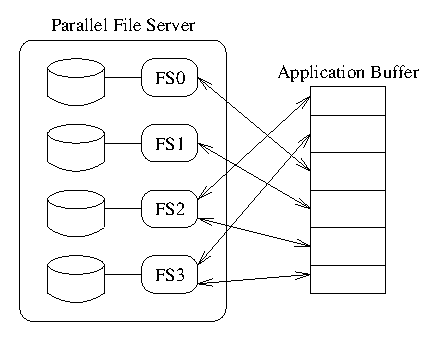
\includegraphics{file.eps}}
\caption{Parallel File Server}
\label{fig:file}
\end{figure}

When an application establishes a connection to the parallel file
server, it will allocate a portal and access control list entry for
communicating with the server.  The access control list entry will
include the portal and match any process in the parallel file server's
group, so all of the file server processes will have access to the
portal.  The portal information and access control entry will be sent
to the file server at this time.  If the application and server need
to have multiple, concurrent I/O operations, they can use additional
portals or match entries to keep the operations from interfering with
one another.

When an application initiates an I/O operation, it first builds a
memory descriptor that describes the memory region involved in the
operation.  This memory descriptor will enable the appropriate
operation (put for read operations and get for write operations) and
enable the use of remote offsets (this lets the servers decide where
their data should be placed in the memory region).  After creating the
memory descriptor and linking it into the appropriate portal entry,
the application sends a read or write request (using \emph{PtlPut}) to
one of the file server processes.  The file server processes can then
use put or get operations with the appropriate offsets to fill or
retrieve the contents of the application's buffer.  To know when the
operation has completed, the application can add an event queue to the
memory descriptor and add up the lengths of the remote operations
until the sum is the size of the requested I/O operation.

\subsection{Dealing with Dropped Requests}\label{sec:exdrop}

If a process does not anticipate unexpected requests, they will be
discarded.  Applications using the Portals API can query the dropped
count for the interface to determine the number of requests that have
been dropped (see Section~\ref{sec:nistatus}).  While this approach
minimizes resource consumption, it does not provide information that
might be critical in debugging the implementation of a higher level
protocol.

To keep track of more information about dropped requests, we use a
memory descriptor that truncates each incoming request to zero bytes
and logs the ``dropped'' operations in an event queue.  Note that the
operations are not dropped in the Portals sense, because the operation
succeeds.

The following code fragment illustrates an implementation of this
approach.  In this case, we assume that a thread is launched to
execute the function \texttt{watch_drop}.  This code starts by
building an event queue to log truncated operations and a memory
descriptor to truncate the incoming requests.  This example only
captures ``dropped'' requests for a single portal.  In a more
realistic situation, the memory descriptor would be appended to the
match list for every portal.  We also assume that the thread is
capable of keeping up with the ``dropped'' requests. If this is not
the case, we could use a finite threshold on the memory descriptor to
capture the first few dropped requests.

\begin{quote}\small
  \begin{cprog}#include <stdio.h>
#include <stdlib.h>
#include <portals.h>

#define DROP_SIZE 32       /* number of dropped requests to track */

int watch_drop( ptl_handle_ni_t ni, ptl_pt_index_t index ) {
    ptl_handle_eq_t drop_events;
    ptl_event_t event;
    ptl_handle_md_t drop_em;
    ptl_md_t drop_desc;
    ptl_process_id_t any_proc;
    ptl_handle_me_t match_any;

    /* create the event queue */
    if( PtlEQAlloc(ni, DROP_SIZE, &drop_events) != PTL_OK ) {
        fprintf( stderr, "Couldn't create the event queue\n" );
        exit( 1 );
    }

    /* build a match entry */
    any_proc.pid_nid = PTL_ADDR_GID;
    any_proc.gid = PTL_ID_ANY;
    any_proc.rid = PTL_ID_ANY;
    PtlMEAttach( index, any_proc, 0, ~(ptl_match_bits_t)0, PTL_RETAIN,
                        &match_any );

    /* create the memory descriptor */
    drop_desc.start = NULL;
    drop_desc.length = 0;
    drop_desc.threshold = PTL_MD_THRESH_INF;
    drop_desc.options = PTL_MD_OP_PUT | PTL_MD_OP_GET | PTL_MD_TRUNCATE;
    drop_desc.user_ptr = NULL;
    drop_desc.eventq = drop_events;
    if( PtlMDAttach(match_any, drop_desc, &drop_em) != PTL_OK ) {
        fprintf( stderr, "Couldn't create the memory descriptor\n" );
        exit( 1 );
    }

    /* watch for "dropped" requests */
    while( 1 ) {
        if( PtlEQWait( drop_events, &event ) != PTL_OK ) break;
        fprintf( stderr, "Dropped request from gid = %d, rid = %d\n",
                   event.initiator.gid, event.initiator.rid );
    }
}\end{cprog}
\end{quote}

\subsection{Message Transmission in MPI}\label{sec:exmpi}

We conclude this section with a fairly extensive example that
describes an approach to implementing message transmission for MPI.
Like many MPI implementations, we distinguish two message transmission
protocols: a short message protocol and a long message protocol.  We
use the constant \texttt{MPI_LONG_LENGTH} to determine the size of a
long message.

For small messages, the sender simply sends the message and presumes
that the message will be received (i.e., the receiver has allocated a
memory region to receive the message body).  For large messages, the
sender also sends the message, but does not presume that the message
body will be saved.  Instead, the sender builds a memory descriptor
for the message and enables get operations on this descriptor.  If the
target does not save the body of the message, it will record an event
for the put operation.  When the process later issues a matching MPI
receive, it will perform a get operation to retrieve the body of the
message.

The following code presents a function that implements the send side
of the protocol.  The global variable \texttt{EndGet} is the last
match entry attached to the portal index used for posting long
messages.  This entry does not match any incoming requests (i.e., the
memory descriptor rejects all get operations) and is built during
initialization of the MPI library.  The other global
variable,\texttt{MPI_NI}, is a handle for the network interface used
by the MPI implementation.

\begin{quote}\small
  \begin{cprog}
extern ptl_handle_me_t EndGet;
extern ptl_handle_ni_t MPI_NI;

void MPIsend( void *buf, ptl_size_t len, void *data, ptl_handle_eq_t eventq,
                    ptl_process_id target, ptl_match_bits_t match ) 
{
    ptl_handle_md_t send_handle;
    ptl_md_t mem_desc;
    ptl_ack_req_t want_ack = PTL_NOACK_REQ;

    mem_desc.start = buf;
    mem_desc.length = len;
    mem_desc.threshold = 1;
    mem_desc.options = PTL_MD_GET_OP;
    mem_desc.user_ptr = data;
    mem_desc.eventq = eventq;

    if( len >= MPI_LONG_LENGTH ) {
        ptl_handle_me_t me_handle;

        /* add a match entry to the end of the get list */
        PtlMEInsert( target, match, 0, PTL_UNLINK, PTL_INS_BEFORE, EndGet, &me_handle );
        PtlMDAttach( me_handle, mem_desc, PTL_UNLINK, NULL );

        /* we want an ack for long messages */
        want_ack = PTL_ACK_REQ;
    }

    /* create a memory descriptor and send it */
    PtlMDBind( MPI_NI, mem_desc, &send_handle );
    PtlPut( send_handle, want_ack, target, MPI_SEND_PINDEX, MPI_AINDEX, match, 0 );
}\end{cprog}
\end{quote}

The \emph{MPISend} function returns as soon as the message has been
scheduled for transmission.  The event queue argument,
\texttt{eventq}, can be used to determine the disposition of the
message.  Assuming that \texttt{eventq} is not \texttt{PTL_EQ_NONE}, a
\texttt{PTL_EVENT_SENT} event will be recorded for each message as the
message is transmitted.  For small messages, this is the only event
that will be recorded in \texttt{eventq}.  In contrast, long messages
include an explicit request for an acknowledgement.  If the
\texttt{target} process has posted a matching receive, the
acknowledgement will be sent as the message is received.  If a
matching receive has not been posted, the message will be discarded
and no acknowledgement will be sent.  When the \texttt{target} process
later issues a matching receive, the receive will be translated into a
get operation and a \texttt{PTL_EVENT_GET} event will be recorded in
\texttt{eventq}.

Figure~\ref{fig:mpi} illustrates the organization of a match list for
receiving MPI messages.  The match list starts with entries that match
the preposted MPI receives (these entries are not shown in
Figure~\ref{fig:mpi}); followed by a match entry that rejects all
incoming requests, called the \emph{RcvMark}; followed by two match
entries that match all incoming requests.  The last two match entries
are used for unexpected messages, i.e., messages that do not match any
of the receives that have been posted by the local MPI process.  The
first of these handles short messages by saving the body of the
message, while the second handles long messages by discarding the
message body.  All of the memory descriptors associated with these
match entries share a common event queue to ensure that unexpected
messages are processed in arrival order.

\begin{figure}[htbp]
\centerline{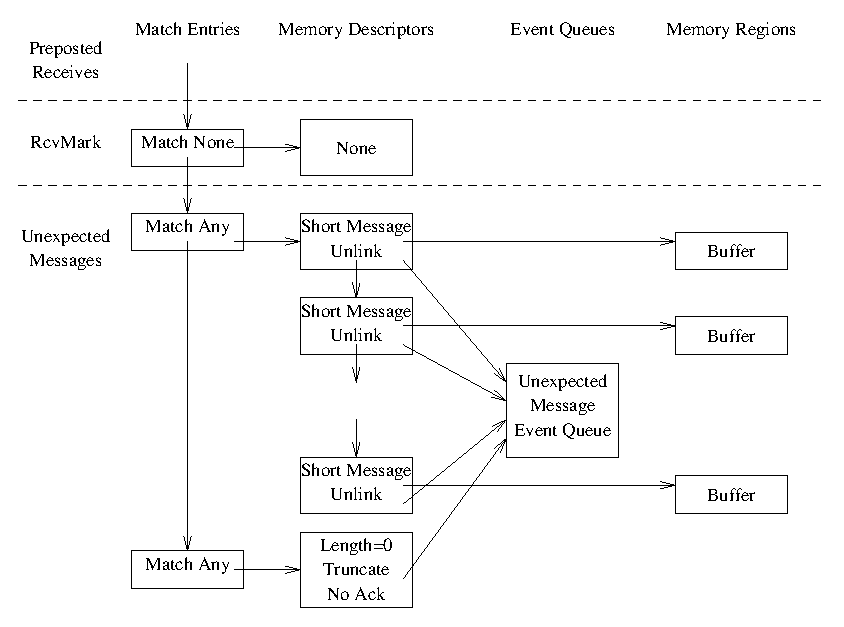
\includegraphics{mpi.eps}}
\caption{Message Reception in MPI}
\label{fig:mpi}
\end{figure}

When the local MPI process posts an MPI receive, a new match entry is
inserted before the \emph{RcvMark} entry and, as such, after all of
the previously posted receives.  This ensures that preposted receives
are matched in the order that they were posted (a requirement of MPI).
Inserting an entry for a preposted receive is not a matter of simply
inserting a match entry before the \emph{RcvMark}.  You must first
check to see if a matching message has arrived before adding the new
entry to match list.  The trick is to avoid the race condition that
results from the possibility that a matching message arrives after you
have searched the match list, but before you have inserted the
preposted receive.  The function presented in

The following code presents a function that avoids this race
condition.  The code starts by creating a memory descriptor and a
match entry which is inserted before the \emph{RcvMark}.  Because the
memory descriptor's \texttt{threshold} is initially set to zero, the
memory descriptor will not respond to any incoming operations.  After
inserting the new match entry, the code searches for a matching
message that has already been received.  If a match is found, the
memory descriptor and match entry are released and the function
returns.  Otherwise, the code conditionally updates the
\texttt{threshold} member of the memory descriptor.  The update is
predicated by the condition that no unexpected messages have arrived
since the start of the search.

\begin{quote}\small
    \begin{cprog}
extern ptl_handle_eq_t UnexpQueue;
extern ptl_handle_me_t RcvMark;
extern ptl_handle_me_t ShortMatch;

typedef struct event_list_tag {
    ptl_event_t           event;
    struct event_list_tag *next;
} event_list;

extern event_list Rcvd;

void AppendRcvd( ptl_event_t event )
{
    /* append an event onto the Rcvd list */
}

int SearchRcvd( void *buf, ptl_size_t len, ptl_process_id_t sender, ptl_match_bits_t match,
                       ptl_match_bits_t ignore, ptl_event_t *event )
{
    /* Search the Rcvd event queue, looking for a message that matches the requested message.
     * If one is found, remove the event from the Rcvd list and return it. */
}

typedef enum { RECEIVED, POSTED } receive_state;

receive_state CopyMsg( void *buf, ptl_size_t length, ptl_event_t event, ptl_md_t md_buf )
{
    ptl_md_t md_buf;
    ptl_handle_me_t me_handle;

    if( event.rlength >= MPI_LONG_LENGTH ) {
        PtlMDBind( MPI_NI, md_buf, &md_handle );
        PtlGet( event.initiator, MPI_GET_PINDEX, 0, event.match_bits, MPI_AINDEX, md_handle );
        return POSTED;
    } else {
        /* copy the message and recycle the buffer */
        memcpy( buf, event.md_desc.start, len );
        event.md_desc.threshold = 1;
        PtlMDAttach( ShortMatch, event.md_desc, PTL_UNLINK, NULL );
        return RECEIVED;
    }
}

receive_state MPIreceive( void *buf, ptl_size_t len, void *MPI_data, ptl_handle_eq_t eventq, 
                                   ptl_process_id_t sender, ptl_match_bits_t match, ptl_match_bits_t ignore )
{
    ptl_md_t md_buf;
    ptl_handle_md_t md_handle;
    ptl_handle_me_t me_handle;
    ptl_event_t event;

    /* build a memory descriptor for the receive */
    md_buf.start = buf;
    md_buf.length = len;
    md_buf.threshold = 0;     /* temporarily disabled */
    md_buf.options = PTL_MD_PUT_OP;
    md_buf.user_ptr = MPI_data;
    md_buf.eventq = eventq;

    /* see if we have already received the message */
    if( SearchRcvd(buf, len, sender, match, ignore, &event) )
         return CopyMsg( buf, length, event, md_buf );

    /* create the match entry and attach the  memory descriptor */
    PtlMEInsert(sender, match, ignore, PTL_UNLINK, PTL_INS_BEFORE, RcvMark, &me_handle);
    PtlMDAttach( me_handle, md_buf, PTL_UNLINK, &md_handle );

    md_buf.threshold = 1;
    do
        if( PtlEQGet( UnexpQueue, &event ) != PTL_EQ_EMPTY ) {
            if( MPIMatch(event, match, ignore, sender) ) {
                PtlMDUnlink( md_handle );  /* don't leave the receive posted */
                return CopyMsg( buf, len, event, md_buf );
            } else {
                AppendRcvd( event );
            }
        }
    while( PtlMDUpdate(md_handle, NULL, &md_buf, unexp_queue) == PTL_NOUPDATE );
    return POSTED;
}\end{cprog}
\end{quote}

\newpage

\begin{center}
{\large\bf References}\vskip -0.4in
\end{center}

\bibliographystyle{ieee}

\bibliography{portals3}

\newpage
\noindent
{\bf Distribution:}
\begin{tabbing}
MM\=MMMMMMM\=MMMMMMMMMMMMMMMMMMMMMMMM\=MMMMMMMMMMM\=\kill
\\
1 \> MS 0321 \> W.\ J.\ Camp, 9200 \\
1 \> MS 0841 \> P.\ J.\ Hommert, 9100 \\
1 \> MS 0318 \> G.\ S.\ Davidson, 9201 \\
1 \> MS 0318 \> P.\ D.\ Heermann, 9215 \\
1 \> MS 1111 \> S.\ S.\ Dosanjh, 9221 \\
1 \> MS 1110 \> D.\ E.\ Womble, 9222 \\
1 \> MS 1110 \> N.\ D.\ Pundit, 9223 \\
1 \> MS 0321 \> A.\ L.\ Hale, 9224 \\
1 \> MS 1111 \> G.\ S.\ Hefflefinger, 9225 \\
1 \> MS 0847 \> R.\ W.\ Leland, 9226 \\
1 \> MS 0819 \> J.\ Peery, 9231 \\
1 \> MS 0820 \> P.\ Yarrington, 9232 \\
1 \> MS 0806 \> L.\ \ Stans, 4616\\
2 \> MS 0899 \> Technical Library, 4916 \\
1 \> MS 9018 \> Central Technical Files, 8940--2 \\
1 \> MS 0612 \> Review and Approval Desk, 4912 \\
  \>         \> For DOE/OSTI \\
\end{tabbing}

\end{document}

